\documentclass[english]{sig-alternate}
\usepackage{amstext}
\usepackage{pdfpages}
\usepackage{alltt}
\usepackage{epstopdf}
\usepackage{xspace,colortbl}
\usepackage[USenglish]{babel}
\usepackage{multirow}
\usepackage{subfigure}
\usepackage{graphicx}
\usepackage{amssymb}
\usepackage{fmtcount}
\usepackage{amsfonts}
\usepackage{xspace}
\usepackage{amsmath}
\usepackage{multirow}
\usepackage[mathscr]{eucal}
%\usepackage{psfrag}
\usepackage{colortbl}
\usepackage{bm}
\usepackage[nospace]{cite}
\makeatletter
\newif\if@restonecol
\makeatother
\let\algorithm\relax
\let\endalgorithm\relax
\usepackage[lined,boxed,vlined,ruled]{algorithm2e}
\special{papersize=8.5in,11in}



\setcounter{secnumdepth}{3}

\long\def\comment#1{}
%\usepackage[dvipdfm]{hyperref}
%\usepackage[dvips]{hyperref}
\begin{document}
\conferenceinfo{SIGMOD'14,} {June 22--27, 2014, Snowbird, Utah, USA.}
\CopyrightYear{2014}
\clubpenalty=10000
\widowpenalty = 10000

%\hyphenpenalty=5000
\tolerance=1000

%\pagenumbering{arabic}

\title{Less is More: Improving Sampling-based Approximate Query Processing with Data Cleaning}

%Identifying Similarity Functions from Examples for Effective Record Matching

%\subtitle{[Extended Abstract]
%\titlenote{A full version of this paper is available as
%\textit{Author's Guide to Preparing ACM SIG Proceedings Using
%\LaTeX$2_\epsilon$\ and BibTeX} at
%\texttt{www.acm.org/eaddress.htm}}}
%\pagenumbering{arabic}

\newtheorem{theorem}{Theorem}
\newtheorem{example}{Example}
\newtheorem{definition}{Definition}
\newtheorem{proposition}{Proposition}
\newtheorem{lemma}{Lemma}
\newtheorem{corollary}{Corollary}

\newcommand{\dataset}{data set\xspace}
\newcommand{\datasets}{data sets\xspace}
\newcommand{\biascorrected}{BiasCorrected\xspace}
\newcommand{\bias}{\biascorrected}
%\newcommand{\sampledirty}{\texttt{SampleDirty}\xspace}
%\newcommand{\sampleclean}{\texttt{SampleClean}\xspace}
%\newcommand{\allclean}{\texttt{AllClean}\xspace}
%\newcommand{\alldirty}{\texttt{AllDirty}\xspace}
\newcommand{\sampledirty}{{SampleDirty}\xspace}
\newcommand{\sampleclean}{{SampleClean}\xspace}
\newcommand{\allclean}{{AllClean}\xspace}
\newcommand{\alldirty}{{AllDirty}\xspace}
\newcommand{\projx}{\textsc{BlinkCrowdDB}\xspace}
\newcommand{\saqp}{SAQP\xspace}
\newcommand{\saqpplus}{SAQP$^{+}$\xspace}
\newcommand{\blinkdb}{BlinkDB\xspace}
\newcommand{\ctable}{\ensuremath{T^{clean}}\xspace}
\newcommand{\var}{\ensuremath{\texttt{var}}\xspace}

\newcommand{\attr}[1]{\texttt{#1}\xspace}
\newcommand{\afunc}[1]{\texttt{#1}\xspace}
\newcommand{\M}{\ensuremath{M}\xspace}
\newcommand{\Pset}{\ensuremath{P}\xspace}
\newcommand{\gfunc}{\ensuremath{f}\xspace}
\newcommand{\avgfunc}{\ensuremath{\texttt{avg} }\xspace}
\newcommand{\varfunc}{\ensuremath{\texttt{var} }\xspace}
\newcommand{\productfunc}{\ensuremath{\texttt{product} }\xspace}
\newcommand{\geomeanfunc}{\ensuremath{\texttt{geomean} }\xspace}
\newcommand{\countfunc}{\ensuremath{\texttt{count} }\xspace}
\newcommand{\sumfunc}{\ensuremath{\texttt{sum} }\xspace}
\newcommand{\groupby}{\ensuremath{\texttt{group-by}}\xspace}
\newcommand{\PCset}{\ensuremath{P^{(c)}}\xspace}
\newcommand{\PCseti}[1]{\ensuremath{P^{(c)}_{#1}}\xspace}
\newcommand{\SCset}{\ensuremath{S}\xspace}
\newcommand{\Sset}{\ensuremath{S}\xspace}
\newcommand{\Pseti}[1]{\ensuremath{P_{#1}}\xspace}
\newcommand{\Sseti}[1]{\ensuremath{S_{#1}}\xspace}
\newcommand{\di}[1]{\ensuremath{d_{#1}}\xspace}

\newcommand{\Correct}[1]{\texttt{Correct}\ensuremath(#1)\xspace}
\newcommand{\Remove}[2]{\texttt{Remove}\ensuremath(#1, #2)\xspace}
\newcommand{\Dedup}[2]{\texttt{Dedup}\ensuremath(#1, #2)\xspace}


\def\indistHIGH{\,{\buildrel d \over \rightarrow}\,} 

%\newcommand{\reminder}[1] {{{\bf [[[#1]]]}\xspace}}
\newcommand{\reminder}[1] {}
\pagestyle{plain}





\maketitle
\thispagestyle{plain}



% A category with the (minimum) three required fields
%\category{H.4}{Information Systems Applications}{Miscellaneous}
%A category including the fourth, optional field follows...
%\category{D.2.8}{Software Engineering}{Metrics}[complexity measures, performance measures]
%\terms{Delphi theory}
%\keywords{ACM proceedings, \LaTeX, text tagging}

% !TEX root = demo.tex
\begin{abstract}
%The prevalence of dirty data presents a fundamental obstacle to modern data-driven applications.
Analysts report spending upwards of 80\% of their time on problems in data cleaning.
The data cleaning process is inherently iterative, with evolving cleaning workflows that 
start with basic exploratory data analysis on small samples of dirty data, then refine analysis with 
more sophisticated/expensive cleaning operators (e.g., crowdsourcing), and finally apply the insights to a full dataset.
While an analyst often knows at a logical level what operations need to be done, they often have 
to manage a large search space of physical operators and parameters.
We present \sys, a system designed to support the iterative development and optimization of data cleaning workflows, especially ones that utilize the crowd.
\sys separates logical operations from physical implementations, and driven by analyst feedback, suggests optimizations and/or replacements to the analyst's choice of physical implementation.
We highlight research challenges in sampling, in-flight operator replacement, and crowdsourcing. 
We overview the system architecture and these techniques, 
then provide a demonstration designed to showcase how \sys can improve iterative data analysis
and cleaning. 
The code is available at: \url{http://www.sampleclean.org}.
\end{abstract}


% !TEX root = demo.tex
\section{Introduction}\label{sec:intro}

\begin{figure}[t]
\centering
\vspace{-0.5cm}
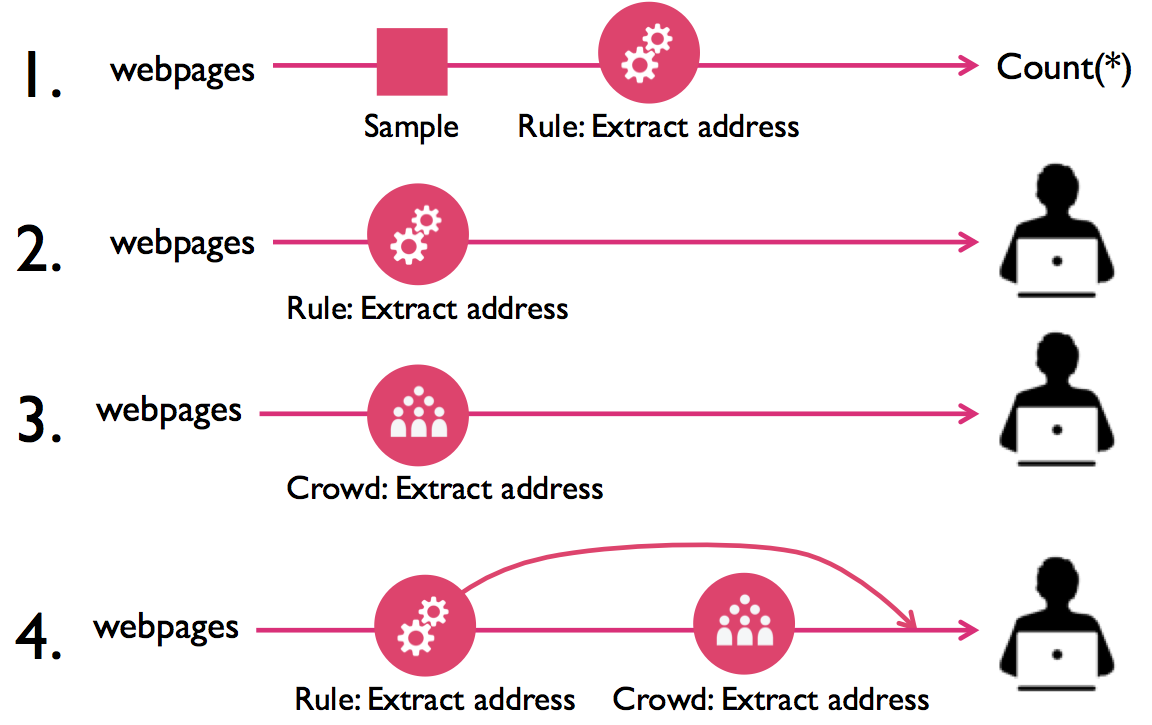
\includegraphics[width = .4\textwidth]{figs/lifecycle.png}
\vspace{-0.4cm}
\caption{Example iterations on the design of the portion of a cleaning plan that extracts restaurant addresses from their unstructured webpages.  
1) An exploratory plan that uses a sample to evaluate a simple address extraction method.
2) A plan that applies the method to the entire dataset. The quality is unsatisfactory. 
3) An alternate plan that uses manual crowd extraction. The quality is now high, but the crowd-based extractor is slow. 
4) A hybrid plan that sends only difficult webpages to the crowd, maximizing accuracy without sacrificing latency.}
\label{fig:ex-plan}
\vspace{-0.3cm}
\end{figure}
% why feedback loops exist/are important (cite Joe’s shit in the past 3 years, blinkdb, etc.). highlight domain specificity. Large variety of data cleaning tasks

%
% General comment that data cleaning is important:
%
The ease of acquiring and merging many large-scale data sources has led to a prevalence of dirty data.
Unfortunately, blindly using results that are derived from dirty data can lead to hidden yet significant errors in modern data-driven applications, so data must be cleaned before it is used.
But because data cleaning is often specific to the domain, dataset, and eventual analysis, analysts report spending upwards of 80\% of their time on problems in data cleaning~\cite{kandel2012}.
The analyst is faced with a breadth of possible errors that are manifest in the data and a variety of options to resolve them.
She must go through the cleaning process via trial and error, deciding for each of her data sources what to extract, how to clean it, and whether that cleaning will significantly change results.

Data cleaning is inherently iterative and Figure~\ref{fig:ex-plan} shows a common progression for the development of a data cleaning plan, in this case the extraction of a restaurant's address from its unstructured webpage.
While this operation can easily be represented at a \textit{logical} level by its input and output schema, there is a huge space of possible \textit{physical} implementations of the logical operators. 
For example, extraction could depend on manually specified rules (\textit{rule-based}), use models trained on previously extracted ground truth records (\textit{learning-based}), ask crowd workers to extract the desired data fields (\textit{crowd-based}), or some combination of the three (e.g., active learning, which uses crowd workers to provide labels for a learning-based approach).
Even after selecting (say) a crowd-based operator, many parameters might influence the quality of the output data or the speed and cost of cleaning: the number of crowd workers who vote on the extraction for a given webpage, the amount each worker is paid, etc.
A priori, a data analyst has little intuition for what physical plan will be optimal in this large space.

Note that in the evolution of the data cleaning plan in Figure~\ref{fig:ex-plan}, our data analyst needed to make many decisions manually about the choice of physical operators by reasoning about their latency, accuracy, and cost. 
Making the wrong decision, for example using the crowd when it only marginally improves accuracy, can be very costly.
A general, scalable, and interactive system that supports rapid iteration on candidate plans would greatly aid this process.

%The prevalance of data cleaning systems in both the research and industrial communities --
%Corleone does blah, XXX addresses blah. Nadeef does blah -- speak to the importance of a
%data cleaning framework as part of the modern big data ecosystems. \ewu{include open access of data in argument?} \jn{We also need to take a look at data cleaning systems in industry. }


% why existing systems suck aka related work
% 1. have slow feedback loops (dataset-dependence, …)
% 2. solve very specific data-cleaning tasks
%Since the beginning of data management, systems have been explored by both the research and industrial communities to improve data cleaning efficiency and quality.
Existing systems seldom address the end-to-end iterative data cleaning process described above.
Extract-transform-load (ETL) systems~\cite{informatica,talend,apachefalcon} require developers to manually write data cleaning rules and execute them as long batch jobs, 
and constraint-driven tools allow analysts to define ``data quality rules" and automatically propose corrections to maximally satisfy these rules \cite{DBLP:conf/sigmod/DallachiesaEEEIOT13}.
Unfortunately, neither provide the opportunity for iteration or user feedback, inhibiting the user's ability to rapidly prototype different data cleaning solutions.
Projects such as Wrangler~\cite{wrangler,trifacta} and OpenRefine~\cite{openrefine} support iteration with spreadsheet-style interfaces that enable the user to compose data cleaning sequences by directly manipulating a sample of the data and applying these sequences to the full dataset.
However, they are limited to specific cleaning tasks such as simple text transformations, do not support crowd-based processing at scale, and cannot incorporate user feedback to optimize the physical implementation of the data cleaning sequences.
Crowd-based~\cite{gokhale2014corleone,stonebraker2013data} systems have been proposed to relieve the data analyst of the burden of rule specification or manual cleaning, but are usually specific to a single cleaning task (e.g.,~\cite{gokhale2014corleone,park2014crowdfill,eracer,chen2014integrating}), preventing end-to-end optimization of the entire cleaning plan.
These existing limitations suggest the need for a system that is general enough to adapt to a wide range of data cleaning applications, scales to large datasets, and natively supports fast-feedback interactions to enable rapid data cleaning iteration.

In this paper, we introduce \sys, a system designed to support the iterative development and optimization of data cleaning plans end to end.
\sys allows users to specify declarative data cleaning plans composed of rule-based, learning-based, or crowd-based operators, then iterate rapidly on plans with cost-aware recommendations for improving the accuracy or latency of a plan.
The effects of a plan can be viewed early using sampling and approximate query processing techniques~\cite{wang1999sample}.

Supporting these capabilities requires a combination of careful engineering 
as well as tackling several research challenges:

\squishlist
\item \textbf{Sampling}: We provide sampling as a first-class logical operator for data cleaning plans that tolerate approximation, and use it to speed up iteration on early-stage plans.

\item \textbf{Recommendation}: We recommend cost-aware changes to in-flight cleaning plans that allow users to trade off accuracy and latency, and provide efficient mechanisms for implementing recommended changes without re-executing the plan on already cleaned tuples.

\item \textbf{Crowd Latency}: We leverage techniques for straggler mitigation~\cite{venkataraman2014power} and model crowd worker speed and accuracy to reduce the (often rate-limiting) latency of crowd data cleaning, consistently retrieving results in seconds rather than hours.
\squishend

In our demonstration, we will run an entity resolution plan on two restaurant datasets, and
show how \sys can be used to 1) specify, modify, and execute a data cleaning plan,
2) quickly clean a sample to characterize how a plan is performing, and
3) observe the same cleaning plans running on multiple datasets.
Users can execute plans over a live crowd that uses the audience as workers, or a simulated crowd
that uses pre-collected crowd responses. The dashboard (Figure~\ref{screenshot}) also provides a live inspection
interface to view the status of the cleaning plan as it executes.

\vspace{-0.2cm}
%Our contributions/requirements
%different ways to tighten the feedback loop:
%end-to-end latency/cost (operator optimization)
%looking versus touching
%Adding introspection (more points of observation)
%hot-swapping (more points of changing plans)
%We have built an end-to-end data cleaning framework with these requirements in mind. (... things we do …) (... engineering contributions …).
%In this demonstration, we highlight the benefits of improving feedback loops for data cleaning using X datasets by optimizing a data cleaning pipeline for one data set/cleaning task, then quickly fitting the pipeline to another dataset.


\if{0}

\jn{Honestly, I didn't quite buy declarativity of the system. In my opinion, data cleaning is so domain specific. It's hard to make it declarative. For a given domain, people may need to write their own data cleaning system. There is a lack of a data cleaning framework that they can build based on. This motivates us to develop such framework. 


We analyze a large variety of domain specific data cleaning systems, and identify several key components: declarative data cleaning operators (e.g., similarity joins), active learning, and crowd/expert sourcing platforms that they require. In our framework, we abstract these components, and implement them in a general way. 

We mainly address two challenges: extensibility and scalability. For the former one, we came up with a nice data-cleaning pipeline API, which people can easily use to compose their own data cleaning tasks. For the latter one, we address it in two aspects: Sampling + Asynchrony.}

\ewu{That's fair, will need to address why a framework is necessary and what benefits it provides.  I think a framework is the correct pitch, hard to sell a set of operators.  Are the above challenges -- extensibility and scalability -- actually difficult?  Worried it's straightforward application of existing techniques.}



In contrast, our work is based on the observation that the majority of data cleaning workflows
can be decomposed into a small set of logical operations (in addition to traditional database operators):
filter based on constraints, extract new fields from existing data, and a similarity join to match
similar or duplicate records. \ewu{quickly validate why this observation holds.} \jn{Yes! I also found that Sec 2.3 has more operators than you describe here.}  
By designing a system around these core operators, we can provide a vast library of physical  
data cleaning operators that span the range of algorithmic, machine learning, and human computation-based
implementations that are necessary practical data cleaning pipelines.   \ewu{Describe live inspection as 
a core feature or is it too easy?}

Designing such a system requires tackling several design challenges:

\begin{enumerate}
\item Speed
\item Quality
\item API Design/extensibilty
\end{enumerate}



We have implemented an initial version of \sys on top of the AMPLab Spark stack, which provides us 
with access to its advanced distributed processing and machine learning features.  Our goal for the current
version is to implement the core mechanisms for declarative specification of the
data cleaning pipeline, solidify the API design, and incle support for, and implementations of,
multiple classes of physical data cleaning operators.


\fi



\if{0}

Cleaning, pre-processing, and formatting data is a required first step in any data analytics pipeline.
However, despite this importance, large-scale data analytics platforms such as Spark or Hadoop lack integrated data cleaning frameworks.
There are a few challenges in building a general purpose data cleaning framework: (1) data cleaning is often
domain specific and requires specialized software targeted at one or a handful of data sources \cite{wang1999sample}, (2) data cleaning is often 
expensive as it increasingly involves human effort via crowdsourcing or experts \cite{DBLP:conf/sigmod/GokhaleDDNRSZ14}, and (3) learning how to clean dirty data from examples
is often hard without a greatly restricted set of operators \cite{DBLP:conf/uist/GuoKHH11}.

We address this problem in \projx by designing a Spark library of composable and scalable data cleaning primitives.
\projx abstracts the logical data cleaning operators: Extraction, Similarity Join, Filtering, from the physical implementation i.e, Rule, Crowd, or Machine Learning.
We interface these primitives through a DSL with which a user can build data cleaning operators that suit their needs.
\projx provides transparent optimizations for each of the components and their composition.
In this demonstration proposal, we present \projx and highlight some of its key features.
While there are many existing systems that do one aspect of data cleaning and transformation (e.g Entity Resolution or Extraction), 
many real world data cleaning tasks have multiple types of errors.
Composing disparate systems can lead to complex code and inefficiencies at scale.
With \projx, we hope to design a set of optimized composable primitives that span a large space of data cleaning tasks.

The first key feature of \projx is that it provides optimized distributed implementations 
of the physical data cleaning operators.
For example, a key step in many deduplication algorithms is a Similarity Join which finds all pairs of records that are within some similarity threshold.
A naive implementation of a Similarity Join would apply a similarity function to all pairs of records.
However, in \projx, we provide optimized implementations of certain common similarity functions (e.g Jaccard, Edit Distance, etc.) that allow for 
a combined broadcast join and prefix filtering which intelligently skips pairs of records using a broadcasted inverted index.

Another feature of \projx is managing the latency and the scale problems of crowd-based data cleaning. 
Crowdsourcing is increasingly prevalent in data cleaning, and \projx provides physical crowd-based implementations
of the logical operators.
However, crowds work at a different latency and scale point in comparison to distributed analytics platforms.
To address the latency problem, we build asychrony into the system.
The user can query intermediate results at any time as crowd responses stream in.
To address the scale issue, \projx provides sampling primitives.
The glue that ties all of the crowd components together is a Machine Learning technique called Active Learning.
As we collect more and more crowd responses, we learn a model that predicts these responses to apply it on the uncleaned data.
Active Learning selects the most informative questions to ask the crowd.

Finally, \projx provides an approximate query processing (AQP) framework.
With slow asynchronous data cleaning algorithms as in crowdsourcing, we need 
to define clear semantics for the intermediate results.
Our AQP framework uses the algorithms proposed in \cite{wang1999sample}, to estimate and bound early results.
It is also common for data scientists to prototype expensive data cleaning pipelines on samples and AQP allows quick evaluation of
aggregate query results on a cleaned sample.

\subsection{Demonstration Scenario}
\reminder{TODO}

\fi




\if{0}
Consider for example, the ability to rapidly understand the types of errors that are present, as well as prevalance of 
these errors is cruicial.



Before an organization can use a new dataset as part of their analysis pipeline
(e.g., to build complex learning models or answer analyst queries)
the errors in the dataset need to be removed in order to ensure accurate conclusions.  

Modern data-driven organizations rely on the ability to ingest and generate large data sets from 
disparate sources, and combine the data together to build complex models or answer analytical questions.  
For example, a restaurant review website may collect restaurant listings by scraping data from webpages or purchasing them from external sources, and
restaurant visitation information for sources such as OpenTable or FourSquare, and aggregate the data to
model user eating habits.  
The set of cleaning tasks necessary for each of these data sources is highly domain and application specific,
and oftentimes the developer is concurrently trying to clean the data source as well as understand its properties.


Oftentimes, these data sources have data quality issues that require a complex data cleaning pipeline -- 
e.g., data extraction, re-formatting, identification and fixes of missing or incorrect values,
and removal of redundant information -- before the data is useable by downstream processes.
Data sources are often domain specific and new for the data analyst, 
As datasets continue to grow, and organizations make use of mure and more datasets, the ability to
rapidly clean the data is more important.  
\fi



\vspace{-.5em}
\section{Query Processing on Dirty Data}\label{sec:error}
Like other \saqp systems, our main focus is on aggregate numerical queries (\avgfunc, \sumfunc, \countfunc, \var, \geomeanfunc, \productfunc) of the form:
\begin{alltt}
SELECT \textsf{f}(attrs) FROM table \\WHERE predicate \\GROUP BY attrs
\end{alltt}
%We defer the implementation of more complex SQL operators such as joins and nested queries for future work.
When running the aggregate queries on large and dirty datasets, there may be two separate sources of errors that affect result quality. (1) Sampling error: since data is large, we may execute queries on a sample of the data to reduce query times. (2) Data error: since real-world data is dirty, queries on the dirty data also lead to inaccurate query results. 

In this section, we first precisely characterize sampling and data errors, and then present our \saqpplus framework to deal with these two types of errors.
Throughout the section, we will refer to the following example query on a dataset of academic publications:
\begin{alltt}
SELECT \textsf{AVG}(citation_count) FROM papers \\GROUP BY pub_year
\end{alltt}
which finds the average number of citations of the publications published every year.

\iffalse
Throughout the section, we will refer to the following example query on a dataset of academic publications:
\begin{alltt}
SELECT \textsf{AVG}(citation_count) FROM papers \\WHERE pub_year>2000
\end{alltt}
which finds the average number of citations received by the publications published after the year 2000.
\fi

\subsection{Sampling Error}\label{subsec:saqp}
There are many different ways to sample data; a data sample could be either created online during the query time~\cite{DBLP:conf/sigmod/HellersteinHW97,DBLP:journals/pvldb/PansareBJC11,DBLP:conf/sigmod/CondieCAHGTES10,DBLP:journals/pvldb/WuJOT09} or built offline from past query workloads~\cite{DBLP:conf/eurosys/AgarwalMPMMS13,DBLP:conf/sigmod/AcharyaGPR99,DBLP:journals/tods/ChaudhuriDN07,DBLP:conf/sigmod/BabcockCD03}.  
Consider our example citation query.
A uniform random-sampling scheme randomly selects a set of papers from \texttt{papers} such that every paper has an equal probability of selection.
%This sampling scheme is not a good choice for a \groupby query since the number of papers published in each year may differ a lot.
%At worst, it will lead to some years with no paper in the sample data.
To answer queries with a highly selective predicate or a \groupby clause, prior works employ stratified-sampling ~\cite{DBLP:conf/sigmod/HellersteinHW97,DBLP:conf/sigmod/AcharyaGP00,DBLP:conf/eurosys/AgarwalMPMMS13}, which performs a uniform random sampling scheme in each group, to guarantee that every group has a large enough sample size to estimate a good result. 
The approaches presented in this paper can support both uniformly random samples and stratified samples.
However, for simplicity, we present our analysis with uniform samples.

Answering queries on a sample has an inherent uncertainty since a different sample may yield a different result.
Quantifying this uncertainty has been extensively studied in statistics~\cite{lohr2010sampling}.
Due to this uncertainty, we return confidence intervals in addition to results.
For example, given a confidence probability (e.g., 95\%), we can apply results from sampling statistics to estimate the average number of citations along with a confidence interval (e.g. $\pm10$), which means that the estimated average number is within $\pm10$ of the actual value with 95\% probability.
The confidence interval quantifies the uncertainty introduced by sampling the data.




%For ease of presentation, we introduce some notations and terminology.

%The basic idea of \saqp is to sample the data, then run the aggregate queries on the sample to obtain approximate results, and finally provide a confidence interval bounding the approximate result.
%Since the query is only run on the sample data instead of the entire data, the query time can be significantly reduced.
%There are two key components of \saqp systems: sample creation and result estimation.
 
%\vspace{.5em}

%{\noindent \bf Sample Creation:} According to different application requirements, a data sample could be either created online during the query time~\cite{DBLP:conf/sigmod/HellersteinHW97,DBLP:journals/pvldb/PansareBJC11,DBLP:conf/sigmod/CondieCAHGTES10,DBLP:journals/pvldb/WuJOT09} or built offline based on query workloads~\cite{DBLP:conf/eurosys/AgarwalMPMMS13,DBLP:conf/sigmod/AcharyaGPR99,DBLP:journals/tods/ChaudhuriDN07,DBLP:conf/sigmod/BabcockCD03}. In comparison, the online sampling has more flexibility to derive an estimate result while the offline sampling can save the sampling time from the query time. 
%
%Consider the query in the beginning of this section. A simple-random-sampling scheme is to randomly select a set of papers from \texttt{papers} such that every paper has the equal probability of the selection. This sampling scheme is not a good choice for a \groupby query since the number of papers published in each year may differ a lot. At worst, it will lead to some years with no paper in the sample data. To avoid this problem, the prior works typically adopt a stratified-sampling scheme~\cite{DBLP:conf/sigmod/HellersteinHW97,DBLP:conf/sigmod/AcharyaGP00,DBLP:conf/eurosys/AgarwalMPMMS13}, which performs a simple-random-sampling scheme in each group, to guarantee that every group has a large enough sample size to estimate a good result. 
%In our paper, we choose the online sampling since we will use the crowd to clean the sample, and the query time is mainly dominated by the crowd-cleaning time. Next, we introduce how to use the online sampling to create a sample for a \groupby query. 


\subsection{Data Error}\label{subsec:dataclean}
In this work, we focus on three types of data errors: \verror, \cerror, and \derror.
We use our example query to illustrate how these errors can affect results.
%Let $\gfunc_{a}(\cdot)$ denote an aggregation function, where $a$ represents an aggregation attribute. (We will often omit $a$ in the function if it is clear from the context.) For example, the aggregation function, $\avgfunc_{\textrm{citation}}(\Pset)$, computes the average number of citations of the papers in $\Pset$.  

%sample data $\Sseti{i}$ randomly drawn from $\Pseti{i}$. For each tuple $t\in \Sseti{i}$, we model its cleaning results as follows:

\vspace{.5em}

\begin{figure}[tup] % \vspace{-1em}
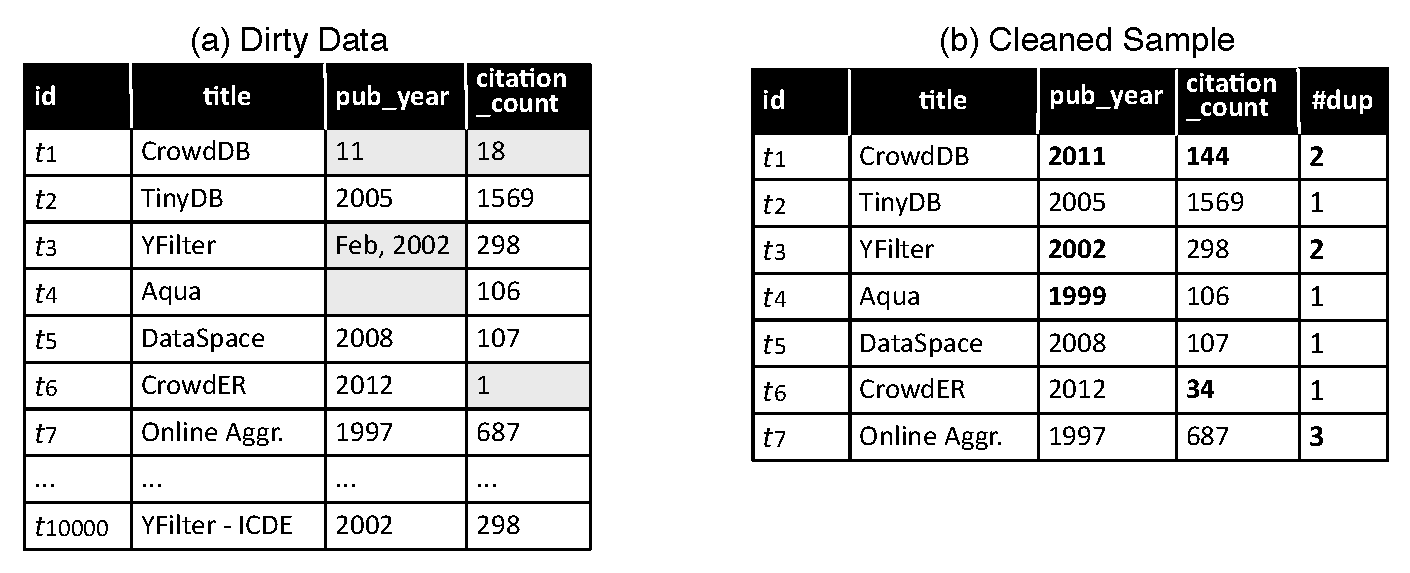
\includegraphics[scale=0.35]{figs/new-example.pdf}\vspace{-1em}
\caption{An example of dirty data and cleaned sample (Shaded cells denote dirty values, and their cleaned values are in bold font).}\vspace{-1.5em}
\label{fig:example}
\end{figure}

{\noindent \bf \Verror:} When an error occurs in the aggregation attributes of the query (i.e. \texttt{citation\_count}), it will lead to an incorrect aggregate result. For example, consider the dirty data in Figure~\ref{fig:example}(a). The first paper $t_1$ involves \verror since its citation count should be 144 instead of 18. %We use $\Correct{t}$ to denote the tuple's correct aggregation-attribute value.  


%Many data-cleaning techniques, such as outlier detection~\cite{hellerstein2008quantitative,DBLP:conf/pervasive/JefferyAFHW06} or rule-based approaches~\cite{fan2012foundations,DBLP:conf/sigmod/DallachiesaEEEIOT13}, have been proposed. We use $\Correct{t}$ to denote the correct aggregation-attribute value of the tuple $t$.  

\vspace{.5em}

{\noindent \bf \Cerror:} When an error occurs in the predicate or group-by attribute of the query (i.e. \texttt{pub\_year}), there may be some tuples that are \emph{falsely} added into or excluded from a group, leading to an incorrect result. In Figure~\ref{fig:example}(a), the first paper $t_1$ also has \cerror since it was published in the year 2011 rather than 11. %Note that this type of error can also be extended to errors in \groupby attributes (refer to Section \ref{sec:query-processing} for details).

%We use $\Predicate{t}$=True ($\Predicate{t}$=False) to denote the cleaned tuple satisfy (dissatisfy) the predicate.


\vspace{.5em}

{\noindent \bf \Derror:} If data contains duplicate tuples (e.g., different representations of the same paper), the aggregate result will also be affected. This type of error commonly happens when the data is integrated from multiple sources. For instance, in Figure~\ref{fig:example}(a), the third paper $t_3$ has \derror as it refers to the same paper as $t_{10000}$.  %We use $\Dedup{t}{\Pset}$ to denote the number of duplicate tuples of $t$ in the dirty data (including $t$ itself).

\vspace{.5em}




%The errors rate (fraction of tuples affected) can vary as well. In this work, we classify \emph{error regimes} by the error rate ranging from 0\% (all of the tuples clean) to 100\% (all of the tuples dirty) for each type of error. Accordingly, we explore how these different regimes affect aggregate query results and our choice of estimation method.

%\Verror and \cerror are both caused by the incorrect attribute values of the dirty data. Many data-cleaning techniques, such as outlier detection~\cite{hellerstein2008quantitative,DBLP:conf/pervasive/JefferyAFHW06} or rule-based approaches~\cite{fan2012foundations,DBLP:conf/sigmod/DallachiesaEEEIOT13}, have been proposed to solve this problem. For example, Fan et al.~\cite{DBLP:journals/pvldb/FanLMTY10} proposed editing rules, master data and user confirmation to correct attribute values, and they proved that their approaches can always obtain reliable cleaning results.

%There are also many studies in dealing with the duplication error (see~\cite{DBLP:journals/tkde/ElmagarmidIV07} for a survey). Particularly, recent work explores the use of crowdsourcing to solve this problem. For example, Wang et al.~\cite{DBLP:journals/pvldb/WangKFF12} proposed a hybrid human-machine framework, which first adopts machine-based techniques to filter obviously non-duplicate tuples for each tuple, and then utilizes the crowd to check the remaining ones. 

While data cleaning can fix the data errors, cleaning the entire data is usually time consuming, often requiring user confirmation or crowdsourcing. For this reason, we have developed the \saqpplus framework.















%Therefore, if it is possible to only clean a sample of the data (i.e., correct the attribute values in the sample, and find the number of duplicate tuples for each tuple in the sample), all of the above .


%Note that the main focus of this work is not on a specific data-cleaning. our work is orthogonal to data-cleaning technique to use. In fact, 




%Note that to compute $\Dedup{t}{\Pset}$, we do not need to compare $t$ with every tuple in the data. Most existing deduplication approaches first employ machine-based techniques~\cite{journals/tkde/Christen11} to identify a candidate set of tuples for $t$, and then only compare $t$ with the candidate tuples. Typically, the number of candidate tuples is much smaller than the whole data size, and scales well with large data sets.




%It is worth mentioning that the above cleaning results cannot capture the missing tuples of the population, i.e. \emph{false-negative error}. For example, there might be some papers that were actually published by ``UC Berkeley" after 2000, but due to the errors in their ``year" or ``university" attributes (e.g., ``year" values are missing or ``UC Berkeley" is represented as ``UCB"), they were not added into the population. As it is hard to know which tuples are missing in the population, in our paper, we assume there is no false-negative error in the population. In practice, to avoid false-negative error, users can create a population by adding all \emph{possible} tuples in it, and transform false-negative error into false-positive error. For example, they can assume all the missing ``year" values satisfy the predicate, and add the corresponding papers (e.g., $t_3$ and $t_4$ in Figure~\ref{fig:example}) into the population. Although some papers may be falsely added into the population, they can use the data-cleaning techniques for the false-positive error to remove such papers (e.g., $t_4$). 

%We assume users should handle such error by themselves. For example, when issuing the query, users can add ``\texttt{or year is NULL}" into the predicate to include the papers whose ``year" values are missing, and then utilize the crowd cleaning (i.e., $\Remove{t}{\Pseti{i}}$) to remove the falsely included papers. They can also identify different representations of ``UC Berkeley" in the ``university" attribute, and add the corresponding tuples into the population w.r.t ``UC Berkeley". Note that the distinct number of \groupby keys is typically much smaller than the number of tuples in the data.

\iffalse
When running the above query on a dirty table, we may get a different result than running on the real clean one. In this section, we analyze what types of data errors will affect the query result, and classify them into three classes: 

\mbox{}

{\noindent \bf Aggregation Error:} When there are incorrect values in aggregate attributes, we call such error as aggregation error. For example, consider the query in Example 1. The citation of Paper 2 in Table 1 is an aggregation error since citation is an aggregate attribute, and the citation number is incorrect and should be 234.


\vspace{.5em}

{\noindent \bf Predicate Error:} Predicate error is caused by the incorrect values in predicate attributes. There are two types of predicate errors: false positive error and false negative error. The former one refers to the tuples that violate the predicate, but falsely identify as satisfying the predicate. The latter one refers to the tuples that satisfy the predicate, but falsely identify as violating the predicate.  



\vspace{.5em}


{\noindent \bf Duplication Error:} 

\mbox{}


Three types of data errors:
\begin{itemize}
  \item {\bf Aggregation Error:} Incorrect values in aggregation attributes
  \item {\bf Predicate Error:} The tuples that satisfy the predicate in the query may not be what users want.
  \item {\bf Duplication Error:} Duplicate tuples in the data
\end{itemize}
\fi

\iffalse
\subsection{Problem Formulation}\label{subsec:problem}
Now we formulate our problem in this section. Given a set of populations that may contain data errors, by cleaning more data, we can estimate a better aggregation result. Since it is expensive to clean the entire data, we investigate how to achieve satisfied result quality by only cleaning a sample of data. Specifically, we study the following two problems:

\vspace{.5em}

{\noindent \bf Quality-constrained problem:} We allow users to specify a constraint of result quality, and aim to clean the minimum number of tuples to satisfy the constraint. The result-quality constraint is defined as an error bound along with a confidence probability. Note that our goal is to estimate the aggregation result for each cleaned population rather than the original (dirty) population. Let $\PCseti{i}$ ($i\in[1,M]$) denote the corresponding cleaned population to $\Pseti{i}$. When we say the estimated result satisfies the quality constraint, it means that the error bar of the estimated result of each $\PCseti{i}$ ($i\in[1,M]$) is smaller than the given error bound with the confidence probability. We formulate this problem as follows:

\begin{definition}
Given a set of populations, an aggregation function, an aggregation attribute, and a result-quality constraint, the goal of quality-constrained problem is to clean the minimum number of tuples in order to make the estimated result of each cleaned population satisfy the quality constraint.
\end{definition}


\vspace{.5em}

{\noindent \bf Cost-constrained problem:} We also allow users to specify a constraint of cleaning cost, and aim to achieve the best result quality within the cleaning cost. The cleaning-cost constraint is defined as the total number of tuples that can be cleaned. For each population, if we can clean more tuples, its result can be estimated more accurately. Therefore, in order to better balance the result quality of different populations, we define the overall quality of all populations as the worst one (with the largest error bar) among them, and study how to determine the number of tuples cleaned for each population to minimize the largest error bar. We formulate this problem as follows:



\begin{definition}
Given a set of populations, an aggregation function, an aggregation attribute, and a cleaning-cost constraint, the goal of cost-constrained problem is to estimate a result for each cleaned population in order to achieve the best overall quality within the cleaning-cost constraint.
\end{definition}


\begin{example}\label{exa:problem-formulation}
Consider two populations, $\Pseti{1}$ w.r.t ``UC Berkeley" and  $\Pseti{2}$ w.r.t ``Stanford". Suppose we want to compute the average citation of the papers in each population. Thus, the aggregation function is \attr{citation} and the aggregation function is \afunc{AVG}. 

Given a result-quality constraint (e.g., error bound: 1\% and confidence probability: 95\%), we then clean the papers in $\Pseti{1}$ and $\Pseti{2}$ to achieve such quality. For instance, after cleaning 1000 papers in $\Pseti{1}$ and 1500 papers in $\Pseti{2}$, assume the estimated average citation of the cleaned $\Pseti{1}$ (i.e., $\PCseti{1}$) is 200 with $\pm0.8\%$ error bar, and the estimated average citation of $\PCseti{2}$ is 180 with $\pm 3\%$ error bar. Since ``UC Berkeley" has already satisfied the quality constraint (i.e. 0.8\% < 1\%), we can stop to clean its papers. But for ``Stanford", we still need to clean its papers until its error becomes smaller than~1\%. 

Given a cost-quality constraint (e.g., 2500 tuples), we then clean at most 2500 tuples in order to achieve the best overall quality. For the above example, if we clean 1000 papers in $\Pseti{1}$ and 1500 papers in $\Pseti{2}$, based on the definition of the overall quality, it will be equal to 3\% that is the error of ``Stanford". Since the error of ``UC Berkeley" is only 0.8\%, it would be better to reduce the number of cleaned tuples for ``UC Berkeley", and save such tuples to clean more tuples for ``Stanford". 
\end{example}

\fi
\iffalse




When the data is clean, it is easy to estimate the aggregation result based on the sample data using existing approaches. However, when the data becomes dirty, the problem becomes challenging since we need to estimate the aggregation result of the entire clean data based on a sample of cleaned data.

Prior \saqp systems assume data is clean, and utilize existing statistical tools to estimate the result based on the sample data. While the data becomes dirty, 

After the crowd has cleaned the sample data, the key problem is how to estimate the aggregation result of the whole clean data based on the cleaned sample data. Next we formulate this problem.

Let $\PCset$ denote the cleaned population set corresponding to $\Pset$. Let $\gfunc(\cdot)$ denote an aggregation function such as $mean(\cdot)$, $sum(\cdot)$ and $count(\cdot)$. Our goal is to estimate the aggregation result of the whole clean data, i.e., $\gfunc(\PCset[a])$, where $\PCset[a] = \{t[a]~|~t\in\PCset\}$ represents the set of aggregation-attribute values in $\PCset$.

\begin{definition}
Given a sample set $\Sset$ randomly drawn from $\Pset$, the crowd-cleaning results $\Correct{t[a]}$, $\Remove{t}{\Pset}$
$\Dedup{t}{\Pset}$ for each tuple $t\in\Sset$, and a confidence probability, we aim to compute (1) an unbiased estimation result of the entire clean data, and (2) an error bound with the specified confidence probability.
\end{definition}







an error-bound constraint with a confidence value

\begin{definition}
Given $M$ population sets, and a cleaning-cost constraint, \projx aims to decide the number of cleaned tuples for each population set such that the 
\end{definition}


For ease of presentation, we assume the query only has aggregate and predicate attributes in the later text. We discuss how \projx processes the query with grouping attributes in Section~\ref{sec:extension}. 


Users are allowed to add time, cost and quality constraints to the query. BlinkDB~\cite{??} has the query language to support time and quality constraints. We extend its language with the cost constraint. For example, a user may want to get the most accurate result within $t$ minutes by at most cleaning $c$ tuples, then she can run the following query:
\begin{alltt}
SELECT Aggregate(\(A\sb{a}\)) FROM \(T\)
WHERE Predicate(\(A\sb{p}\))
WITHIN COST \(c\) TUPLES, TIME \(t\) MINUTES
\end{alltt}
Or given a quality constraint, a user may want to clean the minimum number of tuples to satisfy the quality constraint, then she can run the following query:
\begin{alltt}
SELECT Aggregate(\(A\sb{a}\)) FROM \(T\)
WHERE Predicate(\(A\sb{p}\))
WITHIN ERROR e\% CONFIDENCE f\% 
\end{alltt}
where the quality constraint (or called error bound) means that the true result is within $\pm e$\% of the reported result with f\% probability. 


\begin{figure*}[htup]
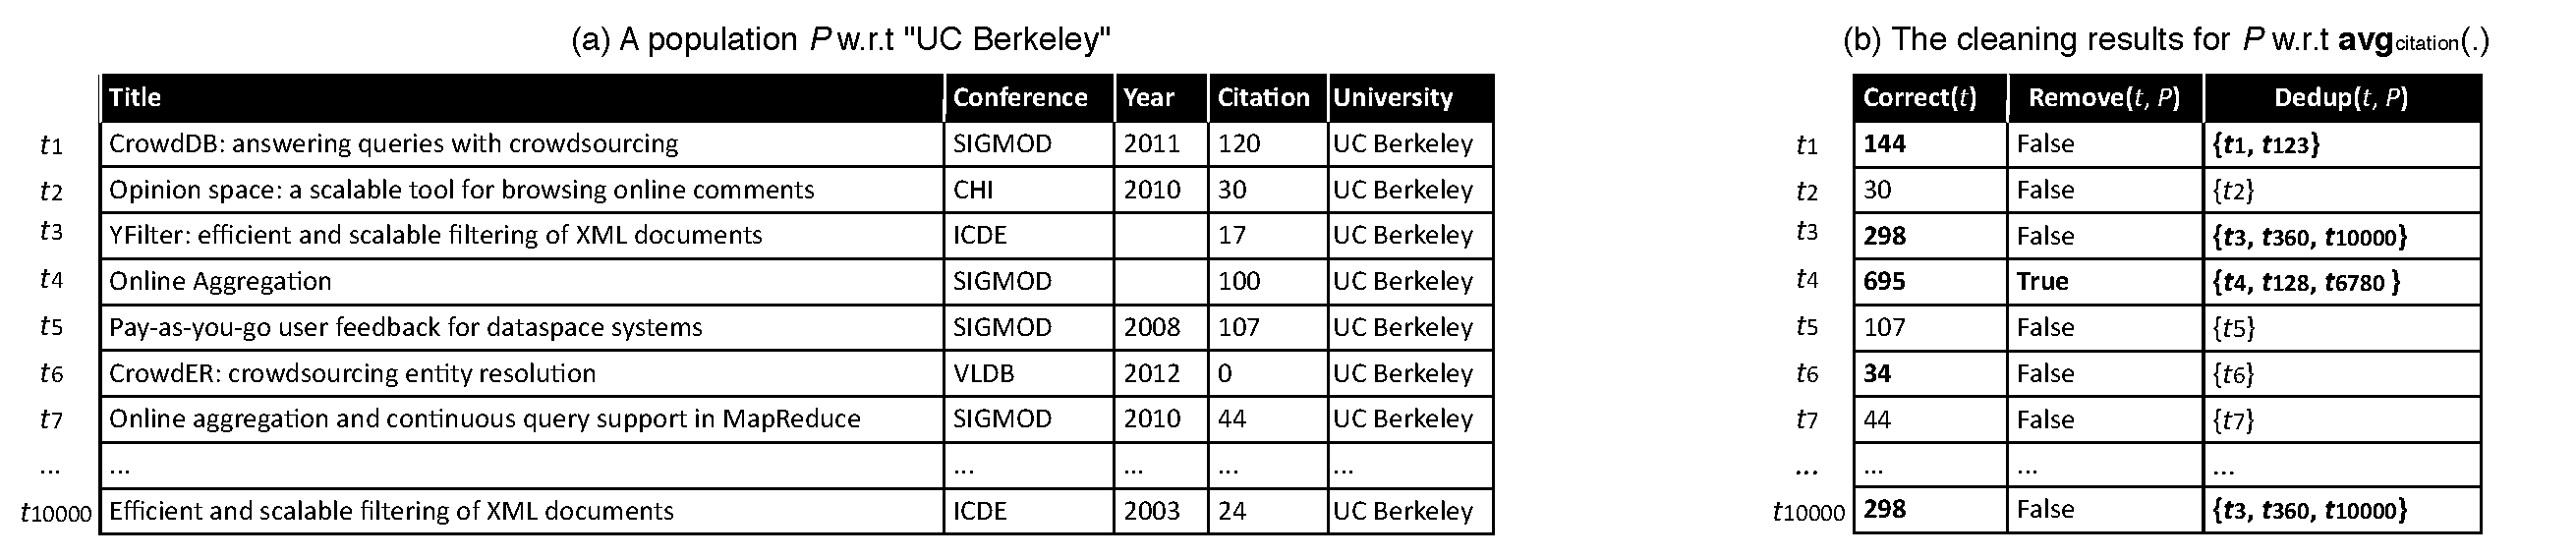
\includegraphics[scale=0.38]{figs/example.pdf}
\caption{A sample of dirty data and the corresponding clean data}
\label{fig:arch}
%\vspace*{-10pt}
\end{figure*}
\begin{example}

\end{example}
\fi
\iffalse
\projx supports a constrained set of SQL \groupby queries, which group tuples in a single table. In addition, \projx also allows users to add the time, cost and quality constraints to the queries. For example, consider the Publication. One example query over the table can be:  
\begin{alltt}
SELECT \textsf{AVG}(Citation) FROM Publication
WHERE year <= 2010
GROUP BY Conference
WITHIN COST 10000 TUPLES, TIME 30 MINUTES
\end{alltt}

    

\begin{alltt}
SELECT Aggregate(\(A\)) FROM Table
WHERE Predicate(\(B\sb{1},B\sb{2},...,B\sb{n}\))
GROUP BY \(C\sb{1},C\sb{2},...,C\sb{m}\)
WITHIN TIME t, ERROR e CONFIDENCE f (, COST c)
\end{alltt}



We start by introducing the BlinkDB extends SQL by enabling 
\begin{itemize}
  \item Group-by query with predicates
  \item Cost/Time/Quality Constraints
  \item \textsf{COUNT}, \textsf{AVG}, \textsf{SUM}, \textsf{STDDEV} and \textsf{VAR}
  \item For example:

  \item Maximize result quality:
  \begin{alltt}
SELECT \textsf{AVG}(Citation) FROM Publication
WHERE Conference = "\textsf{SIGMOD}"
WITHIN COST 1000 TUPLES, TIME 30 MINUTES
\end{alltt}
  \item Minimize cost and time:
  \begin{alltt}
SELECT \textsf{AVG}(Citation) FROM Publication
WHERE Conference = "\textsf{SIGMOD}"
WITHIN ERROR 0.1 CONFIDENCE 95%
\end{alltt}

\end{itemize}

\begin{alltt}
SELECT Aggregate(\(a\)) FROM \(T\)
WHERE Predicate(\(A\sb{p}\))
GROUP BY \(A\sb{g}\),
\end{alltt}

\fi
%Consider the following \groupby SQL query. The query allows users to specify cost, time, and quality constraints. Aggregate function can be \textsf{COUNT}, \textsf{AVG}, \textsf{SUM}, \textsf{STDDEV} and \textsf{VAR}. %To support \groupby queries, we can run the following query for each \groupby key.



%If the quality constraint is not specified, then the query aims to return the highest-quality answer within the cost and time constraints. For example,


%If the quality constraint is specified, then the query aims to spend the least cost and time to return the answer that satisfies the quality constraint. For example,





%WITHIN COST c, TIME t, ERROR e CONFIDENCE f;

%We assume If we are unable to return an answer that satisfies all constraints, we will find the result with the minimum error  Since it may be impossible to get a result that satisfies all constraints, we specify a priority for each constraint, and require that the query has to satisfy the constraints following their priorities. Here we suppose the order of the constraints represent their priorities.



\vspace{-1em}
\section{Framework Overview}\label{sec-arch}
In this section, we formalize the two main problems that \svc addresses: (1) cleaning the staleness errors in a sample of a MV and (2) answering an aggregate query with a clean sample.

\subsection{Notation and Definitions}\label{notation}
In \svc, we explore the problem of approximate aggregate query processing on stale materialized views using a data cleaning approach.
We assume that these materialized views are periodically maintained and thus are stale in between maintenance periods.
The focus of this paper is analytic workloads where the typical query is a group by aggregate on relatively large views.
\svc provides a framework for increased query accuracy for a flexible additional maintenance cost that can scale with system constraints.

%\reminder{You have defined $\mathcal{D}$, $\{R_i\}$, etc in Definition 1. Maybe you can move Def 1 to this Section?}
\noindent \textbf{Materialized View:} Let $\mathcal{D}$ be a database which is a collection of relations $\{R_i\}$. A \emph{materialized view} $S$ is the result of applying a \emph{view definition} to $\mathcal{D}$. 
View definitions are composed of standard relational algebra expressions: Select ($\sigma_{\phi}$), Project ($\Pi$), Join ($\bowtie$), Aggregation ($\gamma$), Union ($\cup$), Intersection ($\cap$) and Difference ($-$). 
We use the following parametrized notation for joins, aggregations and generalized projections:
\begin{itemize}[noitemsep] \sloppy
	\item $\Pi_{a_1,a_2,...,a_k}(R)$: Generalized projection selects attributes $\{a_1,a_2,...,a_k\}$ from $R$, allowing for new columns that are arithmetic transformations of attributes (e.g., $a_1+a_2$).
	\item $\bowtie_{\phi (r1,r2)}(R_1,R_2)$: Join selects all tuples in $R_1 \times R_2$ that satisfy $\phi (r_1,r_2)$. We use $\bowtie$ to denote all types of joins even extended outer joins such as $\rightouterjoin,\leftouterjoin,\fullouterjoin$.
	\item $\gamma_{f,A}(R)$: Apply the aggregate function $f$ to the relation R grouped by the distinct values of $A$, where $A$ is a subset of the attributes.  
	The DISTINCT operation can be considered as a special case of the Aggregation operation. 
\end{itemize}
The composition of the unary and binary relational expressions can be represented as a tree, which is called the \emph{expression tree}.
At the leaves of the tree are all of the \emph{base relations} for a view.
Each node of the tree is the result of applying one of the above relational expressions to a relation.
To avoid ambiguity, we refer to tuples of the base relations as \emph{records} and tuples of derived relations as \emph{rows}.

\noindent \textbf{Primary Key: } We assume that each of the base relations has a \emph{primary key}. If this is not the case, we can always add an extra column 
that assigns an increasing sequence of integers to each record.
For the defined relational expressions, every row in a materialized view can be also be given a primary key \cite{DBLP:journals/vldb/CuiW03, DBLP:conf/sigmod/ZengGMZ14},
which we will describe in Section \ref{sampling}. 
This primary key is formally a subset of attributes $u \subseteq \{a_1,a_2,...,a_k\}$ such that all $s \in S(u)$ are unique.
We denote the entire row for that primary key as a selection $\sigma_u(S)$.

\vspace{.25em}

\noindent \textbf{Staleness: } For each relation $R_i$ there is a set of insertions $\Delta R_i$ (modeled as a relation)
and a set of deletions $\nabla R_i$.
An ``update'' to $R_i$ can be modeled as a deletion and then an insertion.
We refer to the set of insertion and deletion relations as ``delta relations" denoted by $\partial \mathcal{D}$:
\[
	\partial \mathcal{D} = \{\Delta R_1,...,\Delta R_k\} \cup \{\nabla R_1,...,\nabla R_k\}
\]
A view $S$ is considered \emph{stale} when there exist insertions or deletions to any of its base relations.
This means that at least one of the delta relations in $\partial \mathcal{D}$ is non-empty.

\vspace{.25em}

\noindent \textbf{Maintenance: } There may be multiple ways (e.g., incremental maintenance or recomputation) to maintain a view $S$, and we denote the up-to-date view as $S'$.
We formalize the procedure to maintain the view as a \emph{maintenance strategy} $\mathcal{M}$.
A maintenance strategy is a relational expression the execution of which will return $S'$.
It is a function of the database $\mathcal{D}$, the stale view $S$, and all the insertion and deletion relations $\partial \mathcal{D}$. 
In this work, we consider maintenance strategies composed of the same relational expressions as materialized views described above.
\[
S' = \mathcal{M}(S,\mathcal{D}, \partial D)
\]

\vspace{.25em}

\noindent \textbf{Staleness as Data Error: } The consequences of staleness are incorrect, missing, and superfluous rows. 
Formally, for a stale view $S$ with primary key $u$ and an up-to-date view $S'$:
\begin{itemize}[noitemsep] \sloppy
	\item \textbf{Incorrect: } Incorrect row errors are the set of rows (identified by the primary key) that are updated in $S'$: \[\{\forall u \in S : (\exists u \in S' \wedge (\sigma_u(S) \ne \sigma_u(S')))\}\]
	\item \textbf{Missing: } Missing row errors are the set of rows (identified by the primary key) that exist in the up-to-date view but not in the stale view: \[\{\forall u \in S' : \not \exists u \in S\}\]
	\item \textbf{Superfluous: } Superfluous row errors are the set of rows (identified by the primary key) that exist in the stale view but not in the up-to-date view : \[\{ \forall u \in S : \not\exists u \in S' \}\]
\end{itemize}

\vspace{.25em}

\iffalse
\begin{figure}[t] \vspace{-2em}
\centering
 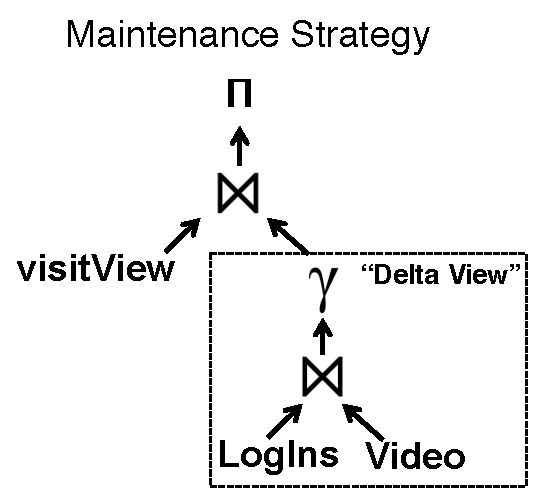
\includegraphics[scale=0.32]{figs/example_expression_tree.pdf} \vspace{-.5em}
 \caption{\reminder{(1). the view definition is different from the one in Sec 2.1; (2) Even if they are the same, it seems not necessary to show it again; (3) Right now you have (b) to show maintenance strategy; maybe you can replace (a) with a figure that shows primary key and ``staleness ad data error"} For our example, we represent the expression tree of the maintenance strategy. We first calculate a delta view using the new insertions and then join this view with the old view.\label{exexpr}}\vspace{-1.5em}
\end{figure}

\vspace{0.45em}
\fi

\noindent \textbf{Uniform Random Sampling: }
We define a sampling ratio $m\in [0,1]$ and for each row in a view $S$, we include it into a sample with probability $m$.
We use the ``hat'' notation (e.g., $\widehat{S}$) to denote sampled relations and sampled relational expressions.
We say the relation $\widehat{S}$ is a \emph{uniform sample} of $S$ if
\[\text{(1) } \forall s \in \widehat{S} : s \in S\text{;~~~~~ (2) }Pr(s_1 \in \widehat{S}) =  Pr(s_2 \in \widehat{S}) = m\]
We say a sample is \emph{clean} if an only if it is a uniform random sample of the up-to-date view $S'$. 

\vspace{0.25em}

\begin{example}\label{concepts}
In this example, we summarize all of the key concepts and terminology pertaining to materialized views, stale data error, and maintenance strategies.
Our example view, visitView, joins the Log table with the Video table and counts the visits for each video grouped by videoId.
Since there is a foreign key relationship between the relations, this is just a visit count for each unique video with additional attributes. 
The primary keys of the base relations are: sessionId for Log and videoId for Video.

If new records have been added to the Log table the visitView is considered stale.
Incorrect rows in the view are videos for which the visitCount is incorrect and missing rows are videos that had not yet been viewed once at the time of materialization. 
While not possible in our running example, superfluous rows would be videos whose Log records have all been deleted.
Formally, in this example our database is $\mathcal{D}=(Video, Log)$, and the delta relations are $\partial\mathcal{D}=(LogIns)$. 

Suppose, we apply the change-table IVM algorithm proposed in \cite{gupta1995maintenance}:
\vspace{-.55em}
\begin{enumerate}[noitemsep]
\item Create a ``delta view" by applying the view definition to LogIns. That is, calculate the visit count per video on the new logs:
\[
 \gamma(Video \bowtie LogIns)
\]
\item Take the full outer join of the ``delta view" with the stale view visitView (equality on videoId).
\[
 VisitView \fullouterjoin \gamma(Video \bowtie LogIns)
\]
\item Apply the generalized projection operator to add the visitCount in the delta view to each of the rows in visitView where we treat a NULL value as 0: 
\[
 \Pi (VisitView \fullouterjoin \gamma(Video \bowtie LogIns))
\]
Therefore, the maintenance strategy is:
\[
 \mathcal{M}(\{VisitView\},\{Video, Log\}, \{LogIns\})
\]
\[
\text{\hspace{0.7em}} = \Pi (VisitView \fullouterjoin \gamma(Video \bowtie LogIns))
\]
\end{enumerate}

\end{example}

%\begin{figure}[t] \vspace{-2em}
%\centering
% 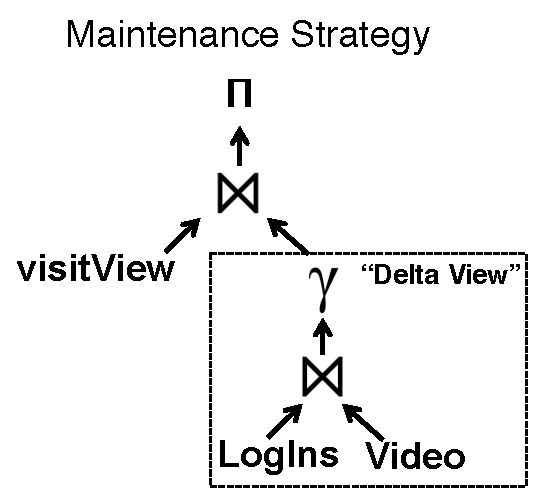
\includegraphics[scale=0.35]{figs/example_expression_tree.pdf} \vspace{-.5em}
% \caption{We illustrate the maintenance strategy of our example view, visitView, in an expression tree. \label{maintstrat}}\vspace{-1.75em}
%\end{figure}

%While, uniform sampling supports a wide variety of query types, it may have issues with queries with highly selective predicates.
%Stratfied sampling has been proposed to mitigate this problem as in the BlinkDB project \cite{AgarwalMPMMS13}.
%However, this requires that we know our query workload in advance.  
%In this paper, we do not discuss stratified sampling and will explore this further in future work.

\subsection{\svc Workflow}
%We summarize the system in Figure \ref{sys-arch} in our introduction.
In this section, we first present an overview of the \svc workflow, and then formalize two challenging problems that we address in the workflow. Formally, the workflow of \svc is:
\begin{enumerate}[noitemsep]
\item We are given a view $S$.
\item $\mathcal{M}$ defines the maintenance strategy that updates $S$ at each maintenance period.
\item The view $S$ is stale between periodic maintenance, and the up-to-date view should be $S'$.
\item \emph{(Problem 1: Stale Sample View Cleaning)} We find an expression $\mathcal{C}$ derived from $\mathcal{M}$ 
that cleans a uniform random sample of the stale view $\widehat{S}$ to produce a ``clean" sample of the up-to-date
view $\widehat{S'}$.
\item \emph{(Problem 2. Query Result Estimation)} Given an aggregate query $q$and the state query result $q(S)$, we use $\widehat{S'}$ and $\widehat{S}$ to estimate the up-to-date result.
\item We optionally maintain an index of outliers $o$ for improved estimation in skewed data.
\end{enumerate} 

\noindent\textbf{Stale Sample View Cleaning: }
The first problem addressed in this paper is how to clean a sample of the stale materialized view.
\begin{problem}[Stale Sample View Cleaning]
We are given a stale view $S$, a sample of this stale view $\widehat{S}$ with ratio $m$, the maintenance strategy $\mathcal{M}$, the base relations $\mathcal{D}$, and
the insertion and deletion relations $\partial \mathcal{D}$.
We want to find a relational expression $\mathcal{C}$ such that:
\[
\widehat{S}' = \mathcal{C}(\widehat{S},\mathcal{D},\partial \mathcal{D})
\]
Where $\widehat{S}'$ is a sample of the up-to-date view with ratio $m$. 
\end{problem}

\noindent\textbf{Query Result Estimation: }
The second problem addressed in this paper is query result estimation.
\begin{problem}[Query Result Estimation]
Let $q$ be an aggregate query of the following form \footnote{\scriptsize For simplicity, we exclude the group by clause for all queries in the paper, as it can be modeled as part of the \textsf{Condition}.}:
\begin{lstlisting} [mathescape,basicstyle={\scriptsize}]
SELECT $agg(a)$ FROM View WHERE Condition(A);
\end{lstlisting}
If the view $S$ is stale, then the result will be incorrect by some value~$c$:
\[
q(S') = q(S) + c
\]
Our objective is to find an estimator $f$ such that:
\[
q(S') \approx f(q(S),\widehat{S},\widehat{S}')
\] 
\end{problem}

\begin{example}\label{infexample}
Suppose a user wants to know how many videos have received more than 100 views.
\begin{lstlisting}[basicstyle={\scriptsize}]
SELECT COUNT(1) FROM visitView WHERE visitCount > 100;
\end{lstlisting}
Let us suppose the user runs the query and result is $45$.
However, there have now been new records inserted into the Log table making this result stale (for clarity no changes to \tbl{Video} or deletions).
First, we take a sample of \tbl{visitView} and suppose this sample is a 5\% sample.

In Stale Sample View Cleaning (Problem 1), we calculate an expression $\mathcal{C}$ based on the maintenance strategy $\mathcal{M}$ described in Example \ref{concepts},
takes the database $\mathcal{D}$ (\tbl{Log} and \tbl{Video}), and the delta relation $\partial \mathcal{D}$ (\tbl{LogIns}).
$\mathcal{C}$ is an optimized relational expression that materializes only a sample of of the updates.
In Query Result Estimation (Problem 2), we take the result of running $\mathcal{C}$ and estimate our above query.
\end{example}

\iffalse
Our query correction component takes the two corresponding samples $\widehat{S'}$ and $\widehat{S}$, and calculates a correction to~$q(S)$.

Like similar restrictions in other sample-based systems \cite{agarwalknowing}, there are restrictions on the queries $q$ on the view that we can answer. 
In the SampleClean work, we focused on \sumfunc, \countfunc, and \avgfunc queries of the form\footnote{\scriptsize For simplicity, we exclude the group by clause for all queries in the paper, as it can be modeled as part of the \textsf{Condition}.}: 
\begin{lstlisting} [mathescape,basicstyle={\scriptsize}]
SELECT $f(a)$ FROM View WHERE Condition(A);
\end{lstlisting}
In this work, we expand the scope of the query processing, and consider general non-nested aggregate queries with predicates.

We also consider correcting stale non-nested select queries of the following form with predicates:
\begin{lstlisting} [mathescape,basicstyle={\scriptsize}]
SELECT * FROM View WHERE Condition(A);
\end{lstlisting}
As with all sample estimates, the accuracy increases with sample size, thus less selective predicates lead to more accurate results.




Note, that this definition is slightly different from the reservoir sampling techniques studied in AQP \cite{DBLP:journals/toms/Vitter85} which find a uniform sample of fixed \emph{size} $k\le \mid S \mid$.
Our sampling ratio gives a sample of the size $k$ in expectation, however, the actual size from any given instance may be slightly different.
For large sample sizes, there is little difference between the techniques since the actual size of using a sample ratio will be close to $k$.
The uniform sample model represents our algorithm which uses hashing better and also makes the presentation of our analysis more clear.

Furthermore, any ``black-box'' uniform sampling algorithm can be used to achieve a reservoir sample.
The use of one technique over another does not affect the general principles or the statistics of \svc, only the 
notation in the analysis.


%\vspace{2em}
\subsection{Problem Statements}
\subsubsection{View Maintenance as Data Cleaning}\label{cleaning}
%In \svc, we model staleness in an MV as a type of data error.
We formalize the problem of correcting staleness as a data cleaning operation so we can apply our data cleaning approach.
In the unsampled case, $\mathcal{M}$ defines a data cleaning operation.
If we are given a materialized view $S$ and we know the base relations have had insertions and deletions, then there are three possible types of error:
(1) a row in $S$ needs to be updated, (2) a row in $S$ needs to be deleted, and (3) new row needs to be inserted into $S$.
Applying $\mathcal{M}$ removes these errors making the view ``clean".
%In the absence of these errors, we call a view \emph{up-to-date}.

However, now suppose we have a sampled view $\widehat{S}$, simply applying updates to the rows in the sample may not suffice.
If new rows need to be inserted into $S$, those will never be represented in the sample violating our uniform sampling.
Thus, we define cleaning in the following way: suppose we have a stale uniform sample $\widehat{S}$, cleaning this sample
should give us $\widehat{S'}$ a uniform sample of the up-to-date view $S'$ with the same sampling ratio.
Formally, this can be represented as the following operations: (1) if an update is needed, update the row, (2) if a row needs to be deleted, delete the row, and (3) for all new rows that need to be inserted into the view $S$ insert a random sample of ratio $m$.

Due to the insertions, the defined data cleaning on a sample does not necessarily give a unique $\widehat{S'}$, so the next question is how to formalize the link between $\widehat{S}$ and $\widehat{S'}$. 
To link a corresponding stale sample (dirty data) and up-to-date sample (clean data), we define the following property:
\begin{definition}[Correspondence]
$\widehat{S'}$ and $\widehat{S}$ are uniform samples of $S'$ and $S$, respectively.  We say $\widehat{S'}$ and $\widehat{S}$ correspond if and only if:
\vspace{-.25em}
\begin{itemize}[noitemsep]
\item For every row $r$ in $\widehat{S}$ that required a delete, $r \not\in \widehat{S'}$
\item For every row $r$ in $\widehat{S}$ that required an update to $r'$, $r' \in \widehat{S'}$
\item For every row $r$ in $\widehat{S}$  that was unchanged, $r \in \widehat{S'}$
\item For every row $r$ in $S$ but not in $\widehat{S}$, $r \not\in \widehat{S'}$
\end{itemize}
\vspace{-.25em}
%\item For every row $r$ in $S'$ that is newly inserted, $r \not\in \widehat{S}$.
%\item If a row $r$ requires an update and then a deletion. The deletion takes precedence and $r \not\in \widehat{S'}$.
%\item Rows that are inserted trivially satisfy the conditions since those rows are not contained in $S$ or $\widehat{S}$.
\label{correspondence}
\end{definition}
%This definition of correspondence gives us a way to get two samples from which we can take a row-by-row difference.
%There is some nuance in how to handle null values which we discuss in Section \ref{correction}.

The goal of \svc is to efficiently produce a corresponding up-to-date sample from a stale one thus cleaning the sample.
In the first component of \svc (Section \ref{sampling}), we take as input a uniform sample of a stale view $\widehat{S}$, a maintenance strategy $\mathcal{M}$, and a set of updates $\{\Delta R_i\} \cup \{\nabla R_i\}$.
We return $\widehat{S'}$, a clean uniform sample (a uniform sample of $S'$) that satisfies the correspondence property with $\widehat{S}$.

\iffalse

\begin{example}[Correspondence]
Suppose \tbl{countView} has 4 video rows: 
\begin{lstlisting} [mathescape]
V1 (visitCount = 4), V2 (visitCount = 6), V3 (visitCount = 1), V4 (visitCount = 1)
\end{lstlisting}
We take a sample of \tbl{countView} and call it \tbl{countViewSample} that contains V1 and V2.
\tbl{LogIns} has new logs of 1 visit for V1 and 1 visit for a new video V5.
An up-to-date sample that corresponds is:
\begin{lstlisting} [mathescape]
V1 (visitCount = 4+1), V2 (visitCount = 6)
\end{lstlisting}
An up-to-date sample that does \emph{not} corresponds is: 
\begin{lstlisting} [mathescape]
V1 (visitCount = 4+1), V3 (visitCount = 1)
\end{lstlisting}
This is because V2 was unchanged and therefore should be included in the sample.
\end{example}
\fi

\subsubsection{Query Result Correction}
In the query result correction phase, we take a query result on a stale view and use the up-to-date sample to compensate for the staleness.
Given a query $q$ which has been applied to the stale view $q(S)$ giving a stale result.
Our query correction component takes the two corresponding samples $\widehat{S'}$ and $\widehat{S}$, and calculates a correction to~$q(S)$.

Like similar restrictions in other sample-based systems \cite{agarwalknowing}, there are restrictions on the queries $q$ on the view that we can answer. 
In the SampleClean work, we focused on \sumfunc, \countfunc, and \avgfunc queries of the form\footnote{\scriptsize For simplicity, we exclude the group by clause for all queries in the paper, as it can be modeled as part of the \textsf{Condition}.}: 
\begin{lstlisting} [mathescape,basicstyle={\scriptsize}]
SELECT $f(a)$ FROM View WHERE Condition(A);
\end{lstlisting}
In this work, we expand the scope of the query processing, and consider general non-nested aggregate queries with predicates.

We also consider correcting stale non-nested select queries of the following form with predicates:
\begin{lstlisting} [mathescape,basicstyle={\scriptsize}]
SELECT * FROM View WHERE Condition(A);
\end{lstlisting}
As with all sample estimates, the accuracy increases with sample size, thus less selective predicates lead to more accurate results.
%From these queries, we exclude the group by clause, as we model group by clauses as part of the \textsf{Condition}.
\fi

\iffalse
\subsubsection{Outlier Indexing}
The query correction in the previous subsection is derived from a sample.
Sampling is known to be sensitive to outliers, which we define as records whose values deviate significantly from the mean.
However, a challenge is that since we do not materialize the entire up-to-date view detecting which records may be outliers is challenging.
Instead, we define an outlier index on base relations of the database $\mathcal{D}$.
This index tracks records whose attributes cross some threshold $t$.
Then, for a given view $S$, this component gives a series of rules to propagate the information from the outlier index upwards.
Basically, for every row in the view that is derived from a record in the outlier index, we ensure that it is incorporated into the sample.
We use the set of outliers to return a more accurate correction result.
\fi
%We explore the conditions under which we can make this guarantee, and discuss query processing with the outlier index in Section \ref{outlier}.


\iffalse
\subsection{Example Application}
Returning to our example \tbl{countView}, suppose a user wants to know how many videos have received more than 100 views.
\begin{lstlisting}[basicstyle={\scriptsize}]
SELECT COUNT(1) FROM visitView 
WHERE visitCount > 100;
\end{lstlisting}
Let us suppose the initial query result is $45$.
There now have been new log records inserted into the Log table making the old result stale.
For example, if our sampling ratio is 5\%, that means for 5\% of the videos (distinct \tbl{videoId}), we update just the view counts of those videos.
Suppose 2 videos have changed their counts from less than 100 to greater than 100.
%From this sample, we calculate how many new videos changed from less than 100 views to times greater than 100; let us suppose this answer is $2$.
%Since our sampling ratio is 5\%, 
From this sample, we extrapolate that $40$ new videos throughout the view should now be included in the count.
This means that we should correct the old result by $40$ resulting in the estimate of $45+40 = 85$.
\fi



\section{\sampleclean Estimation}\label{sec:sampleclean}
In this section, we present the \sampleclean estimation approach.
\sampleclean takes a sample of data as input, applies a data cleaning technique to the sample, runs an aggregate query directly on the clean sample,
and returns a result with a confidence interval.

\subsection{Sample Estimates}\label{subsec:resultestimation}
We will first introduce the estimation setting without data errors and explain some results about estimates from sampled data.
We start with the table of $N$ tuples which we call $P$, the \emph{population}.
From $P$, we sample a subset $S$ of size $K$ uniformly; that is, every tuple is sampled with equal probability.
In this setting, we have two problems: (1) Estimate an aggregate query result on the sample $S$; (2) Quantify the uncertainty of the query result.

Consider a simpler problem; suppose we want to estimate the \mean value of $P$.
We can calculate the \mean of $S$ and the Central Limit Theorem (CLT) states that these estimates follow a normal distribution:
\begin{equation}\small
N(\mean(P),\frac{var(P)}{K})
\end{equation}
Since the estimate is normally distributed, we can define a confidence interval parametrized by $\lambda$ (e.g., 95\% indicates $\lambda=1.96$)\footnote{\scriptsize When estimating means of finite population there is a finite population correction factor of $FPC=\frac{N-K}{N-1}$ which scales the confidence interval.}.
\begin{equation}\small
\mean(S) \pm \lambda \sqrt{\frac{var(S)}{K}}.
\end{equation}
This interval has two interpretations: (1) if we re-compute the \mean value on another random sample, the result will be within the confidence interval with the specified probability, and (2)
the true value $\mean(P)$ is within the confidence interval with the specified probability.
Furthermore, we call this estimate \emph{unbiased} since the expected value of the estimate is equal to the true value.

Our primary focus is answering \avgfunc, \countfunc, and \sumfunc queries with predicates\footnote{\scriptsize Group-by queries can be implemented by adding group-by keys into predicates.} (see~\cite{saqpfull} for other queries).
We can estimate these queries by re-formulating them as \mean value calculations.
We first define some notation:
\begin{itemize}\vspace{-.5em}
\item $f(\cdot)$: a function representing any of the supported aggregate queries with a predicate.
\item \Predicate{t}: the predicate of the aggregate query, where \Predicate{t} = 1 or 0 denotes $t$ satisfies or dissatisfies the predicate, respectively.
\item $K$: the number of tuples in the sample.
\item $K_{\pred}$: the number of tuples that satisfy the predicate in the sample.
\item $t[a]$: the aggregation-attribute value. If it is clear from the context that $t$ refers to an attribute value rather than a tuple, we will omit `$[a]$' for brevity.

\end{itemize}
We can reformulate all of the queries as calculating a \mean value so we can estimate their confidence intervals with the CLT:
\begin{equation}\label{eq:general-func}\small
f(S) = \frac{1}{K} \sum_{t \in S} \saqpfunc(t)
\end{equation}
where $\saqpfunc(\cdot)$ expresses all of the necessary scaling to translate the query into a \mean value calculation:
\begin{itemize}\vspace{-.5em}
\item \countfunc: $\saqpfunc(t) = \Predicate{t} \cdot N$\vspace{-.5em}
\item \sumfunc: ~\, $\saqpfunc(t) = \Predicate{t} \cdot N \cdot t[a]$\vspace{-.5em}
\item \avgfunc: ~\, $\saqpfunc(t) = \Predicate{t} \cdot \frac{K}{K_{\pred}}  \cdot t[a] $ 
\end{itemize}
For example, the \avgfunc query is estimated from the sample as:
\begin{equation}
\avgfunc(S) = \frac{1}{K_{pred}}  \sum_{t \in S} \Predicaten{t} \cdot t[a],
\end{equation}
which computes the average value of the tuples that satisfy the predicate in the sample. In order to represent $\avgfunc(S)$ in the form of Equation~\ref{eq:general-func}, we rewrite it to the following equivalent Equation:  
\begin{equation}
\avgfunc(S) = \frac{1}{K}  \sum_{t \in S} \Predicaten{t} \cdot \frac{K}{K_{\pred}}  \cdot t[a].
\end{equation}
Therefore, we have $\saqpfunc(t) = \Predicate{t} \cdot \frac{K}{K_{\pred}}  \cdot t[a] $ for the \avgfunc query.


\iffalse
A key feature of this formulation is the case statement, \Predicate{t}, where tuples that do not satisfy the predicate set the entire term for that tuple by 0. 
It is important to note is that $f(S)$ is defined as the average of $\saqpfunc(\cdot)$ over all tuples including the 0 values, not just the ones that satisfy the predicate.
It will be clear in the subsequent sections that it is convenient to define $f(S)$ in this way to handle condition errors.
However, we need to be careful about scaling factors for each of the queries.

For the \countfunc query, we calculate the average value of \Predicate{t} over all tuples and scale that by the dataset size N.
In other words, this calculates the fraction of tuples that satisfy the predicate, and then multiplies that by the size of the dataset.
Similarly, for the \sumfunc query, we can extend this by multiplying \Predicate{t} by the value of the tuple.
Consequently, we calculate an average value (including 0's for the tuples that don't satisfy the predicate) and we can scale this by the dataset size N.

The \avgfunc query needs a more complex scaling factor.
Since we are interested in the \avgfunc of all the tuples that satisfy the predicate, we have to calculate: 
\begin{equation}
\frac{1}{K_{pred}}  \sum_{t \in S} \Predicaten{t} \cdot t[a]
\end{equation}
However, our formulation of $f(S)$ uses $\frac{1}{K}$ not $\frac{1}{K_{pred}}$.
We accordingly have to rescale by $\frac{K}{K_{\pred}}$ in \saqpfunc(t).
Intuitively, if we include the 0 values from where \Predicate{t} is false in our average, this will lead to an underestimate of the true average.
So, we need to compensate by a factor of $\frac{K}{K_{\pred}}$.
\fi
\subsection{Unbiased Estimation with Data Errors}
If we ignore data errors, the estimates described in the previous section are unbiased.
Suppose $P_{\clean}$ is the corresponding clean population for the dirty data population $P$.
We are interested in estimating an aggregate query on $P_{\clean}$.
However, since we do not have the clean data, we cannot directly sample from $P_{\clean}$.
We must draw our sample from the dirty data $P$ and then clean the sample.

The key question is whether running an aggregate query on the cleaned sample is equivalent to computing the query result on a sample directly drawn from the clean data.
When this is true, our estimate is unbiased, and we can derive confidence intervals using the CLT.
In the following section, we explore this question on different types of data errors.
Our goal is to define a new function $\saqpplusfunc(\cdot)$, an analog to $\saqpfunc(\cdot)$, that corrects attribute values and re-scales to ensures that the estimate remains unbiased.

Recall, that we model three types of errors: value error, condition error, and duplication error.
To correct the errors, we can define two data cleaning primitive functions:
\begin{itemize}\vspace{-.5em}
\item \Correct{t}: for the tuple t return a tuple with correct attribute values\vspace{-.5em}
\item \Dedup{t}{P}: for the tuple t return the number of times that the tuple appears in the population~$P$ 
\end{itemize}


\subsubsection{Value and Condition Errors}
Both value and condition errors are caused by incorrect attribute values of the dirty data.
These errors do not affect the size of the population, i.e., $|P| = |P_{\clean}|$.
Furthermore, correcting a value or condition error only affects an individual tuple.
Consequently, if we apply the $\saqpfunc(\cdot)$ to the corrected tuple, we still preserve the uniform sampling properties of the sample, $S$.
In other words, the probability that a given tuple is sampled is not changed by our correction of value and condition errors, thus we define $\saqpplusfunc(t)$ as:
\begin{equation}\small
\saqpplusfunc(t) = \saqpfunc \left( \Correct{t} \right).
\end{equation}

Note that the $\saqpfunc(\cdot)$ for an \avgfunc query is dependent on the parameter $K_{\pred}$. 
If we correct values in the predicate attributes, we need to recompute $K_{\pred}$ in the cleaned sample.

\subsubsection{Duplication Error}\label{subsec:challenges}
Since duplication errors affect multiple tuples and the size of $P_{\clean}$ is different from the size of $P$, they do affect the uniformity of the sampling.
The following example illustrates the consequences of duplication errors:
\begin{example}
Consider a population $P = \{t_1, t_2, t'_2\}$ with two distinct tuples, $t_1$ and $t_2$ (=$t'_2$).
If we draw samples of size 2 from this population uniformly:
\[ Pr(\{t_1, t_2\})=\frac{1}{3},\ Pr(\{t_1, t'_2\})=\frac{1}{3},\ Pr(\{t_2, t'_2\})=\frac{1}{3}. \]
Now, assume $t_1 = 1$ and $t_2 = t_2' = 2$.
The expected \mean value over all random samples is $\frac{1}{3}\cdot\frac{3}{2}+\frac{1}{3}\cdot\frac{3}{2}+\frac{1}{3}\cdot2=\frac{5}{3}$, however the cleaned population is $P_{\clean} = \{t_1, t_2\}$ and its \mean value is actually $\frac{3}{2}$. %Thus, when duplication errors exist, it may be biased to estimate a result based on the cleaned sample.
\end{example}
The duplicated data is more likely to be sampled and thus be over-represented in the estimate of the \mean.
We can address this with a weighted mean to reduce the effects of this over-representation.
Furthermore, we can incorporate this weighting into $\saqpplusfunc(\cdot)$.

Specifically, if a tuple $t$ is duplicated $m=\Dedup{t}{P}$ times, then it is $m$ times more likely to be sampled, and we should down weight it with a $\frac{1}{m}$ factor compared to the other tuples in the sample.
We formalize this intuition with the following lemma:
\begin{lemma}\label{lem:derror}
Let $P$ be a population with duplicated tuples. % and $P_{unique}$ be the set of unique tuples.
Let $S \subseteq P$ be a uniform sample of size $K$.
For each $t_{i}\in S$, let $m_i$ denote its number of duplicates in $P$.
 (1) For \sumfunc and \countfunc queries, applying $\saqpplusfunc(t_i)=\frac{\saqpfunc(t_i)}{m_i}$ yields an unbiased estimate;
(2) For an \avgfunc query, the result has to be scaled by the duplication rate $d=\frac{K}{K'}$,
where $K'=\sum_i\frac{1}{m_i}$, so using $\saqpplusfunc(t_i)=d\cdot\frac{\saqpfunc(t_i)}{m_i}$ yields an unbiased estimate.
\end{lemma}

\begin{proof}[sketch] We can interpret the population as a discrete probability distribution, and the sample as drawing $K$ elements from this distribution.
Since some elements are duplicated there is an increased probability of drawing these elements.
We reduce these effects by re-weighting the samples, which can be thought of as drawing fractional samples (i.e., if we sample an element which is duplicated twice, we cancel it out by treating it as sampling only half an element).
As a result, while we may draw $K$ total samples, the total number of fractional samples drawn (sum of the weights) $K'$,
may be different, so we have to scale the result accordingly. See~\cite{saqpfull} for a detailed proof.
\end{proof}
We apply this lemma to the following example:
\begin{example}\label{exa:derror}
Consider the dirty data in Figure~\ref{fig:example}, $P = \{t_1, t_2, \cdots, t_{10000}\}$, and the sample data, $\Sset = \{t_1, t_2, t_3, t_4,$ $t_5, t_6, t_7\}$. In this example, we assume the data only has duplication error, and our goal is to estimate the average citation count of all the papers in the data. 

Firstly, we compute the duplication rate of the sample: 
\[\frac{K}{\sum_{t\in S} \frac{1}{\Dedup{t}{P}}} = \frac{7}{\frac{1}{2}+\frac{1}{1}+\frac{1}{2}+\frac{1}{1}+\frac{1}{1}+\frac{1}{1}+\frac{1}{3}} = 1.31\]

Then, we apply $\saqpplusfunc(\cdot)$ to each paper $t\in \Sset$. Specifically, we divide its citation count by the number of duplicates and then multiple it by the duplication rate, i.e., $\saqpplusfunc(S) = \{\frac{1.31\cdot 18}{2}, \frac{1.31\cdot1569}{1}, \frac{1.31\cdot298}{2}, \cdots , \frac{1.31\cdot687}{3}\}$. For example, the first paper's citation count is 18 and it has two duplicates, thus we have $\saqpplusfunc(t_1) = \frac{1.31\cdot 18}{2}$. 


Finally, we estimate the average citation count as the \mean of $\saqpplusfunc(S)$.

%Firstly, for each paper $t\in \Pset$, we divide its citation count by the number of duplicates, and obtain a set of corrected citation counts for the sample data, i.e., $\saqpplusfunc(S) = \{\frac{18}{2}, \frac{1569}{1}, \frac{298}{2}, \frac{106}{1}, \frac{107}{1}, \frac{1}{1}, \frac{687}{3}\}$.
%Then we take the weighted average of the sample, which is $\frac{1}{7}\cdot (\frac{18}{2}+\frac{1569}{1}+\frac{298}{2}+\frac{106}{1}+\frac{107}{1}+\frac{1}{1}+ \frac{687}{3}) = 310$.


%Therefore, based on Lemma~\ref{lem:derror}, we can estimate the average citation count, i.e., $1.31*310 = 406.1$.
\end{example}

\subsubsection{Combinations of Errors}\label{subsec:comb-challenge}
We can also address data with combinations of errors (e.g., duplicated tuples that also have incorrect values).
Value and condition errors affect a tuple's values.
Duplication errors affect a tuple's sampling probability.
The two classes of errors affect the tuple in different ways, and consequently, we define a single function $\saqpplusfunc(\cdot)$ which can correct for all three error types:


\begin{itemize}\vspace{-.5em}
\item \countfunc: $\saqpplusfunc(t) = \frac{\saqpfunc(\Correct{t})}{\Dedup{t}{P}}$\vspace{-.5em}
\item \sumfunc: ~\, $\saqpplusfunc(t) =\frac{\saqpfunc(\Correct{t})}{\Dedup{t}{P}}$\vspace{-.5em}
\item \avgfunc: ~\, $\saqpplusfunc(t) = d\cdot\frac{\saqpfunc(\Correct{t})}{\Dedup{t}{P}}$ 
\end{itemize}

We plug $\saqpfunc(\cdot)$ (as described in Section~\ref{subsec:resultestimation}) into the above equations, and obtain a more detailed form of $\saqpplusfunc(t)$ as shown in Table~\ref{tbl:transform-new}.
%Let $N$ be the total size of the dataset (including duplicates), $K$ be the size of the sample (including duplicates), $K_{pred}$ be the number of tuples in the sample that satisfy the predicate (including duplicates), and $d$ be the duplication rate estimated from the sample. 
%We get the following transformations:
%For more details about the composability of these functions, see~\cite{saqpfull}.

\iffalse
\begin{table}[htup]\vspace{-1em}
\label{tbl:transform}
\scriptsize
\caption{$\saqpplusfunc(\cdot)$ for \sumfunc, \countfunc, and \avgfunc}
\centering 
\begin{tabular}{l l}
\hline\hline
Query & $\saqpplusfunc(\cdot)$\\
\hline  % inserts single horizontal line
\vspace{.5em}
$\avgfunc$ & $\frac{d\cdot\saqpfunc(\Correct{t})}{\Dedup{t}{P}}
$ \\\vspace{.5em} % inserting body of the table
$\sumfunc$ & $ \frac{\saqpfunc(\Correct{t})}{\Dedup{t}{P}}
$ \\\vspace{.5em}
$\countfunc$ & $
		\frac{\saqpfunc(\Correct{t})}{\Dedup{t}{P}}
$ \\ [1ex] % [1ex] adds vertical space
\hline %inserts single line
\end{tabular}
\end{table}
\fi


\begin{table}[htup]\vspace{-1em}

\small
\caption{$\saqpplusfunc(\cdot)$ for \countfunc, \sumfunc, and \avgfunc. Note that $N$ is the total size of dirty data (including duplicates).}
\centering 
\begin{tabular}{l l}
\hline\hline
Query & $\saqpplusfunc(\cdot)$\\
\hline  % inserts single horizontal line
\vspace{.5em}
$\countfunc$ & $
		\Predicatec{t}\cdot N\cdot\frac{1}{\Dedup{t}{P}}
$ \\\vspace{.5em} % inserting body of the table
$\sumfunc$ & $
		\Predicatec{t}\cdot N\cdot\frac{\Correct{t}[a]}{\Dedup{t}{P}}
$ \\\vspace{.5em}
$\avgfunc$ & $
		\Predicatec{t}\cdot \frac{dK}{K_{\pred}}\cdot\frac{\Correct{t}[a]}{\Dedup{t}{P}}
$ \\ [1ex] % [1ex] adds vertical space
\hline %inserts single line 
\label{tbl:transform-new}
\end{tabular}\vspace{-2em}
\end{table}


\vspace{.5em}
{\noindent \bf \sampleclean Estimation:}
We can now formulate the \sampleclean estimation procedure, as follows:

\begin{enumerate}
\item Given a sample $S$ and an aggregation function $f(\cdot)$\vspace{-.5em}
\item Apply $\saqpplusfunc(\cdot)$ to each $t_i \in S$ and call the resulting set $\saqpplusfunc(S)$\vspace{-.5em}
\item Calculate the mean $\mu_c$, and the variance $\sigma_c^2$ of $\saqpplusfunc(S)$\vspace{-.5em}
\item Return $\mu_c \pm \lambda \sqrt{\frac{\sigma_c^2}{K}}$\vspace{-.5em}
\end{enumerate}

To summarize, we state that the \sampleclean approach gives an unbiased estimate:

\begin{theorem}\label{thm:sampleclean}
Given an aggregation function $f$ and a population $P$,
where there are three types of errors: value, condition, and duplication.
Let S be a uniform sample $S \subseteq P$ of size $K$.
Let $\saqpplusfunc(S)$ be the set of tuples where $\saqpplusfunc(\cdot)$ is applied to every tuple.
Then the estimate on this sample is given by:
\[ \mean \left( \saqpplusfunc(S) \right) = \frac{1}{K}\sum_{t\in S} \saqpplusfunc(t) \]
The estimate is an unbiased estimate of $f(P_{\clean})$.
\end{theorem}
\begin{proof}[sketch]
We need to show that the aggregation $\saqpplusfunc(S)$ is equivalent to the aggregation $\saqpfunc(S_{\clean})$.
Lemma~\ref{lem:derror} shows that this is true for duplication errors.
We further argued that with value errors and condition errors $\saqpplusfunc(S) = \saqpfunc(S_{\clean})$.
Finally, since duplication error correction and value/condition correction can be composed this is true.
As the \mean of a uniform random sample of $P_{\clean}$, this is an unbiased estimate.
See~\cite{saqpfull} for a detailed proof.
\end{proof}

%For each paper $t\in S$, if $t$ is removed from $S$ (i.e. $\Remove{t}{P}$ = True), we set $\phi_f(t) = 0$; otherwise, we first correct its citation number (i.e. \Correct{t}), and then divide the correct citation number by the number of duplicates (i.e., |\Dedup{t}{P}|), and finally obtain its transformed value $\phi_f(t)=\frac{d}{r}\cdot\frac{\Correct{t}}{|\Dedup{t}{P}|}$.
Consider the following end-to-end numerical example with \sampleclean:

\begin{example}\label{exa:sampleclean}
Consider the sample data and the cleaning results in Figure~\ref{fig:sample}, and assume the data may involve three types of errors.
To estimate the query result, we need to map each $t \in S$ to a new value $\saqpplusfunc(t)$.
Since the sample contains seven papers, and $t_4$ and $t_7$ do not satisfy the predicate, the scaling for predicates is $\frac{K}{K_{\pred}} = \frac{7}{5}=1.40$.
As shown in Example~\ref{exa:derror}, the duplication rate is $d = 1.31$.
After applying $\saqpplusfunc(\cdot)$ for \avgfunc query in Table~\ref{tbl:transform-new} to each sampled paper, we obtain the transformed sample data of $\saqpplusfunc(S) = \{133,\, 2895,\, 275,\, 0,\, 197,\, 63,\, 0\}$.
For example, since $t_1$ satisfies the predicate, and its correct citation count is 144 and the number of duplicates is 2, we have $\saqpplusfunc(t_1) = 1.31\cdot 1.40 \cdot\frac{144}{2} = 133$.
Similarly, as $t_4$ does not satisfy the predicate, we have $\saqpplusfunc(t_4) = 0$. 
We calculate the \mean $\mu_c$ and the variance $\sigma_c^2$ of $\saqpplusfunc(S)$, and return $\mu_c \pm \lambda \sqrt{\frac{\sigma_c^2}{K}}$ as the estimated average citation count, where $\lambda$ is a constant value derived from the user-specified confidence probability.
\end{example}

\begin{figure}[t]\vspace{-1em}
\centering
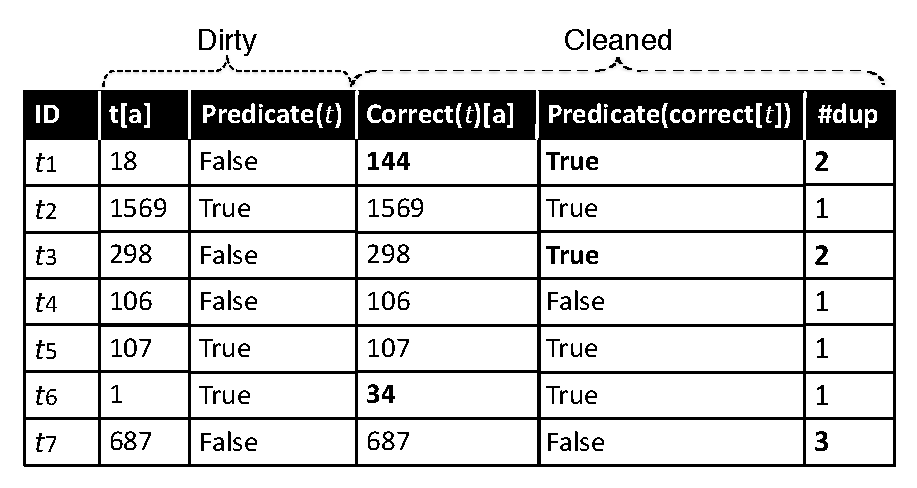
\includegraphics[scale=0.45]{figs/sample.pdf}\vspace{-1em}
\caption{The cleaning results for the sample $\Sset = \{t_1, t_2, t_3, t_4, t_5, t_6, t_7\}$  w.r.t ``SELECT \textsf{AVG}(citation\_count) FROM papers WHERE pub\_year>2000". The values in bold font indicate the changed values after data cleaning.}\vspace{-.5em}
\label{fig:sample}\vspace{-.5em}
\end{figure}

\vspace{.5em}
{\noindent \bf Remarks.} % There are a few additional remarks about \sampleclean. 
%We have mentioned that the \avgfunc query is affected by scaling since its result has to be scaled by the size of the sample.
(1) For an \avgfunc query, we can achieve tighter confidence intervals by skipping the tuples that dissatisfy the predicate instead of considering them as 0 values.
The reason for this is that the \avgfunc query has a scaling factor $r=\frac{K}{K_{\pred}}$, which is a random variable itself.
The confidence intervals we present incorporate the additional variance of~$r$, but due to the skipping we can get estimates not affected by that variance. (2) Algorithmically, we contrast \sampleclean from \saqp with $\saqpplusfunc(\cdot)$ vs. $\saqpfunc(\cdot)$, which makes it very convenient to implement \sampleclean in an existing \saqp system.
%This is particularly convenient for implementation since, if we know the query, we can simply transform the data prior to passing it to an existing \saqp framework.

%The method can obtain unbiased query results along with quality guarantees from the cleaned sample.
%We first introduce a basic theory of sample-based result estimation in Section~\ref{subsec:resultestimation}, and then 
%discuss the new challenges posed by data errors in Section~\ref{subsec:challenges}. We addresses these challenges and present the \sampleclean algorithm in Sections~\ref{subsec:dup-challenge} and~\ref{subsec:comb-challenge}.
%Note that there are other ways (e.g., bootstrapping~\cite{hinkley1988bootstrap}) to compute confidence intervals.
%In principle, we can use other confidence interval techniques, and we illustrates how to use bootstrapping for queries that do not have convenient analytic confidence intervals in~\cite{saqpfull}.


%\begin{lemma}\label{lem:derror}
%Let $P$ be a population with $N$ data tuples, and $P^{c}$ the cleaned population  with $N'$ unique data tuples. For each $p_{i}\in P$, let $m_i$ denote its number of duplicates in $P$ and let $\frac{p_{i}}{m_{i}}$
%represent a data tuple where the aggregation-attribute value is 
%divided by $m_{i}$. Then for the set $\hat{P}^{c}=\{\frac{p_{1}}{m_{1}},\frac{p_{2}}{m_{2}},...,\frac{p_{N}}{m_{N}}\}$,
%the mean value (denoted by $\mathbb{E}(\cdot)$) of the set $\hat{P}^{c}$ is:
%\[
%\mathbb{E}(P^{c})=d\cdot \mathbb{E}(\hat{P}^{c}) 
%\]
%where $d$ is the duplication ratio $\frac{N}{\sum_{i}^{N}\frac{1}{m_{i}}}=\frac{N}{N'}$.
%\end{lemma}
%\begin{proof}[sketch] (See Appendix) We can treat a population as a discrete probability distribution over the values of its aggregation attribute.
%Since $\mathbb{E}(X):=\sum_i iPr(X==i)$, if an attribute with the value i has been duplicated $m$ times then $Pr(X==i)$ is $m$ higher so down weighting
%those attributes by a factor of $m$ compensates for the increase.
%\end{proof}\vspace{-1em}

%As important consequence of this lemma is that we can extend this reasoning to samples and obtain an unbiased estimate.

%\subsection{Combinations of Errors}\label{subsec:comb-challenge}
%In our problem formulation, we discussed two other forms of errors: aggregation errors and predicate errors.
%These can similarly be addressed through design of $\phi^{*}_f(\cdot)$.

%With aggregation errors, the intuitive transformation works where we set an incorrect value to its correct value.
%Since these errors only affect single tuples, the estimate on the transformed data is still unbiased and it is functionally similar to sampling from a data where all the tuples have cleaned aggregation-attribute values.

%Predicate errors are a little bit more complex since they not only affect the value of an aggregation, they also have effects on the size of the sample.
%However, we can use a similar trick as the previous section where rather than removing a tuple that does not satisfy the query predicate, we can set its value to zero.
%Since all of our queries follow additive forms, this means that the tuple does not contribute to the result.

%Similar to scaling problem with duplication errors, the \avgfunc will be off by a proportionality constant $r$, which is the fraction of tuples that satisfy the query.
%We accordingly use the estimate $\hat{r}$, the fraction of tuples in the sample that satisfy the predicate, to maintain the correct scaling. 

%Based on this design of $\phi^{*}_f(\cdot)$, we propose the following:

%\begin{lemma}\label{lem:comp}
%Given an aggregation function $f$,
%let $\phi^{*}_{f(1)}$ be the transformation
%that estimates unbiasedly under duplication
%errors. Let $\phi^*_{f(2)}$ be unbiased
%under predicate errors, and $\phi^*_{f(3)}$
%be unbiased under aggregation errors.
%We can define a composed function $\phi^*_f(\cdot) = \phi^*_{f(2)}(\phi^*_{f(1)}(\phi^*_{f(3)}(\cdot)))$,
%that is unbiased under all three errors.
%\end{lemma}
%\begin{proof}[sketch] 
%We can re-define clean estimation in stages: (1) estimate the function unbiasedly if aggregation errors were the only problem,
%(2) given data that is free of aggregation errors, we fix duplication errors, (3) finally, we remove tuples that do not satisfy the predicate. In this order of operations, the functions are
%composable. See~\cite{saqpfull} for a detailed proof.
%\end{proof}

%As a result, we have a single choice of $\phi^*_f(\cdot)$ as shown in Table~\ref{tbl:transform} that addresses our three types of data errors.
%\subsection{SampleClean Algorithm}

\section{\bias Estimation}\label{sec:biascorrected}
\sampleclean estimates a result directly on a clean sample of data.
The size of confidence intervals in the \sampleclean estimate are function on the variance of
the cleaned sample $var(\saqpplusfunc(S))$ and the sample size $K$.
This property implies that the accuracy of \sampleclean is only dependent on the cleaned values (independent of the magnitude of incorrect values), and thus makes the technique robust to large errors.
This dependence may not be desirable in datasets where the data itself has high variance or where errors are small in magnitude.
%In this case, our desired estimation technique should give more accurate results for the data with small errors. 

This motivates the \bias approach, where we take an existing aggregation of the data, estimate its difference from the true value, and
then use the estimate to correct the existing aggregation.
The resulting technique gives us confidence intervals that are dependent on the variance of the errors, which can allow us to estimate very accurately on datasets
where this variance is small.
Furthermore, we provide the same unbiased guarantees on \bias as \sampleclean.

\subsection{Estimating the Difference}
Due to data errors, the result of the aggregation function~$f$ on the dirty population $P$ differs from the true result by~$\epsilon$:
\[f(P) = f(P_{\clean}) + \epsilon\]
In the previous section, we derived a function $\saqpplusfunc(\cdot)$ for \sampleclean estimation.
We contrasted this function with $\saqpfunc ( \cdot )$ which does not clean the data.
Therefore, we can write:
\begin{equation}
f(P) = \frac{1}{N}\sum_{t\in P}\saqpfunc(t)\hspace{2em}
f(P_{\clean}) = \frac{1}{N}\sum_{t\in P}\saqpplusfunc(t)
\end{equation}
If we solve for $\epsilon$, we find that:
\begin{equation}
\epsilon = \frac{1}{N}\sum_{t\in P}\Big(\saqpfunc(t)-\saqpplusfunc(t)\Big)
\end{equation}
In other words, for every tuple t, we calculate how much $\saqpplusfunc(t)$ changes $\saqpfunc(t)$.
For a sample $S$, we can construct the set of differences between the two functions:
\[\scriptsize
Q=\{\saqpfunc(t_1)-\saqpplusfunc(t_1),\saqpfunc(t_2)-\saqpplusfunc(t_2), \cdots ,\ \saqpfunc(t_K)-\saqpplusfunc(t_K)\}\]
The \mean difference is an unbiased estimate of $\epsilon$, the difference between $f(P)$ and $f(P_{\clean})$.
We can subtract this estimate from an existing aggregation of data to get an estimate of $f(P_{\clean})$.

\vspace{.5em}{\noindent \bf \bias Estimation}
We derive the \bias estimation procedure, which corrects an aggregation result:
\begin{enumerate}
\item Given a sample $S$ and an aggregation function $f(\cdot)$
\item Apply $\saqpfunc(\cdot)$ and $\saqpplusfunc(\cdot)$ to each $t_i \in S$ and call the set of differences  $Q(S)$.
%Set $s_i$ to zero if the tuple does not satisfy the predicate in the dirty data.
\item Calculate the mean $\mu_q$, and the variance $\sigma_q$ of $Q(S)$
\item Return $(f(P) - \mu_q) \pm \lambda \sqrt{\frac{\sigma_q^2}{K}}$
\end{enumerate}

Similar to \sampleclean, we can prove that the result in unbiased:
\begin{theorem}\label{thm:bias}
Given an aggregation function $f$ and a population $P$,
where there are three types of errors: value, condition, and duplication.
Let S be a uniform sample $S \subseteq P$ of size $K$.
Let $Q$ be the set of tuples where $q(t)=\saqpfunc(t)-\saqpplusfunc(t)$ is applied to every tuple.
Then the estimate on this sample is given by:
\[ mean(Q) = \frac{1}{K}\sum_{t\in S} \Big (\saqpfunc(t)-\saqpplusfunc(t) \Big)\]
is an unbiased estimate of the bias $\epsilon$.
It follows, that $f(P)-\epsilon$ is an unbiased estimate of the result.
\end{theorem}
\begin{proof}[sketch] We can apply the theory developed for \sampleclean to the estimate of $\epsilon$.
Since it is unbiased, due to the linearity of expectation the estimate $f(P)-\epsilon$ is also unbiased.
See~\cite{saqpfull} for a detailed proof.
\end{proof}

Consider the Example~\ref{exa:sampleclean} discussed in the previous section.
\begin{example}
Based on the definition of $\saqpfunc(\cdot)$ in Section~\ref{subsec:resultestimation}, we have 
\[\saqpfunc(S) = \{0,\ 3661,\ 0,\ 0,\ 250,\ 2,\ 0\}. \]
For example, as shown in Figure~\ref{fig:sample}, since $t_1$ does not satisfy the predicate, we have $\saqpfunc(t_1) = 0$.
Additionally, as $t_2$ satisfies the predicate, and its dirty citation is 1569 and the scaling for predicates is 
$\frac{K}{K_{\pred}}=\frac{7}{3}$, we have $\saqpfunc(t_2) = \frac{7}{3}\cdot 1569 = 3661$. 

Over the same data we apply $\saqpplusfunc(\cdot)$ (as shown in Example~\ref{exa:sampleclean})  
\[\saqpplusfunc(S) = \{133,\ 2895,\ 275,\ 0,\ 197,\ 63,\ 0\}, \]
we can obtain the difference between the two samples
\[Q(S) = \{-133,\ 766,\ -275,\ 0,\ 53,\ -61,\ 0\}.\]
We calculate the \mean $\mu_q$ and the variance $\sigma_q^2$ of $Q(S)$, and return $(f(P) - \mu_q) \pm \lambda \sqrt{\frac{\sigma_q^2}{K}}$.
\end{example}

\subsection{\bias vs. \sampleclean}
We compare \sampleclean and \bias on result accuracy and processing time.
Both methods achieve unbiased estimates, but may differ greatly in the accuracy (the size of the confidence interval) of these estimates.
The confidence interval of \bias is given by $\pm\lambda\sqrt{\frac{\sigma_q^2}{K}}$ and for \sampleclean it is  $\pm\lambda\sqrt{\frac{\sigma_c^2}{K}}$.
Therefore, for a fixed sample size, if $\sigma_c \ge \sigma_q$, \bias will be more accurate.
In cases when either $\sigma_c$ is large or $\sigma_q$ is small, \bias can give a result with narrower confidence intervals than \sampleclean.
For example, if we had no data errors then $\sigma_q = 0$ (a perfect \bias estimate), but $\sigma_c$ would still be non-zero as it is the variance of the cleaned data.
Conversely, the more unpredictable (high variance in the difference between the clean and dirty data) the error offset is, the worse \bias will perform.

In terms of processing time, \bias is very different from \sampleclean as it needs to run an aggregation query on the entire dataset.
We highlight two situations that are not affected by this additional processing.
(1) When the time required to clean a sample is much larger than the time needed to scan the entire dataset.
(2) When the user has an existing result on the dirty dataset and wants to assess how far away it is from the true value.
In these settings, we can maintain results for both \sampleclean and \bias and return the result with a tighter confidence interval.

The analysis in this section assumes that we can compute an exact aggregation result on the dirty dataset.
We can also extend \biascorrected by estimating the aggregate result based on a sample without accessing the entire data.
In this way, \biascorrected requires less response time but may lose some result accuracy.
Interested readers are referred to~\cite{saqpfull} for details.

%\subsection{Discussion}
%While \sampleclean and \biascorrected are functionally similar, they may differ greatly in the accuracy of their estimates.
%In \bias, the size interval is determined by the variance of the set Q, i.e., $\sigma_q$, not $\sigma_c$ as in \sampleclean.
%In cases when either $\sigma_c$ is large or $\sigma_q$ is small, \bias can give a result with narrower confidence intervals than \sampleclean.
%Conversely, the more unpredictable (high variance in the difference between the clean and dirty data) the error offset is, the worse \bias will perform.
%After already spending the cleaning effort, it is relatively cheap to maintain results for both \biascorrected and \sampleclean, and we can simply report the one with a narrower confidence interval.
%However, as discussed earlier, \bias is only feasible when we can get an exact aggregation result on the dirty data.
%It may not be suited for ad-hoc or interactive applications.
%{\noindent \bf Remark.} When data becomes larger, it might be costly for \biascorrected to obtain an exact aggregate result of the entire dirty data.
 








%\section{Queries and Parameters}
For each of our supported queries, the specifics of the cleaning determine the algorithm parameters.
As discussed in the previous section, we want to construct the functions $\phi(.)$ and $f(.)$ in such a way that we obtain an unbiased estimator and analytic CLT error bars for our desired aggregator.
Recall, that we support three cleaning operations: correcting aggregation errors, identifying false positives, and merging duplicates.
These operations are not mutually exclusive and real data may contain all three types of errors (numerical, false positive, and duplication).

That said, we will incrementally derive the parameters for these operations.
We will start with data that only contains aggregation errors, then consider data that contains both aggregation errors and false positive errors, and finally consider errors that may also include duplication.
The derivation will show the dependencies of the estimators on various aspects of the data independent of other error types (e.g., error variance, false positive rate, duplication rate).  
To keep our data type consistent (tuples vs. numerical attribute), most of the $f(.)$ functions will have a term $t[j]$.
Recall from (Section ???), that this means we are extracting the j-th numerical attribute from the tuple $t$ and we are only considering single dimensional aggregations.

\subsection{Numerical Errors}
First, let us consider the simplest case when the tuples only have aggregation errors.
In this model, we can see that if $\phi(.)$ assigns a correct value to any incorrect tuples $\phi(t_i)= t_i^{(c)}$, then the result will be in expectation the aggregation of the clean data.
\begin{table}[!ht]
\caption{Algorithm Parameters for data with only aggregation errors}
\centering 
\begin{tabular}{c c c c}
\hline\hline
Query & $\phi(.)$ & $f(.)$ \\ 
\hline  % inserts single horizontal line
$\textbf{avg}$ & $\phi(t_i)=t_i^{(c)}$ &$f(t)=t[j]$ \\ % inserting body of the table
$\textbf{sum}$ & $\phi(t_i)=t_i^{(c)}$ & $f(t))=Nt[j]$ \\
$\textbf{count}$ & $\phi(t_i)=t_i^{(c)}$ & $f(t)= N$ \\ [1ex] % [1ex] adds vertical space
\hline %inserts single line
\end{tabular}
\end{table}

\subsection{False Positive Errors}
Now, we can extend the previous analysis to the case when some tuples are false positives.
In this case, we want to make sure we don't include their contributions into the aggregations.
This leads to the intuitive choice of $\phi(.)$, which sets the aggregation attributes of tuples that don't satisfy the predicate to zero.
This means that that \textbf{sum} and \textbf{count} will be correct and the mean will be correct up to a proportionality constant of the fraction of tuples zeroed in the sample $r$.

\begin{table}[!ht]
\caption{Algorithm Parameters for data with aggregation errors and false positive errors}
\centering 
\begin{tabular}{c c c c}
\hline\hline
Query & $\phi(.)$ & $f(.)$ \\ 
\hline  % inserts single horizontal line
$\textbf{avg}$ & $\phi(t_i)=\left\{
	\begin{array}{ll}
		t_i^{(c)}  & \mbox{if } \text{predicate} \\
		0 & \text{otherwise}
	\end{array}
\right.$ & $f(t)=\frac{1}{r}t[j]$ \\ % inserting body of the table
$\textbf{sum}$ & $\phi(t_i)=\left\{
	\begin{array}{ll}
		t_i^{(c)}  & \mbox{if } \text{predicate} \\
		0 & \text{otherwise}
	\end{array}
\right.$ & $f(t)=Nt[j]$ \\
$\textbf{count}$ & $\phi(t_i)=\left\{
	\begin{array}{ll}
		1 & \mbox{if } \text{predicate} \\
		0 & \text{otherwise}
	\end{array}
\right.$ & $f(t)=Nt[j]$ \\ [1ex] % [1ex] adds vertical space
\hline %inserts single line
\end{tabular}
\end{table}

\subsection{Duplication Errors}
Duplication errors are particularly troublesome since they affect the sampling properties of the dataset.
If a tuple has been duplicated, then it will be over represented in random sample.
For our set of supported aggregation functions, we can use a reweighting technique to address the problem of duplication.

A more detailed proof and discussion can be found in the appendix, but for intuition consider the definition of the
discrete expected value function:
\[\mathbb{E}(x)=\sum_{x=-\infty}^{\infty}x\mathbb{P}(X=x) \]
If a data item with value $x$ is duplicated, it affects $\mathbb{P}(X=x)$ by the number of times it has been duplicated $m$.
If we know $m$ we can reweight $x'=\frac{x}{m}$, so that in the aggregation it cancels out the additional contribution.
Basically, the end result is that up-to some scaling we can acheive an estimate that is unbiased even if we merge some duplicate values.

Similar to our definition of $r$ in our discussion of the false positive errors, we introduce a variable $d$ to be the duplication rate of a sample $d=\frac{\text{total}}{\text{unique}}$.

\begin{table}[!ht]
\caption{Algorithm Parameters for data with all three errors}
\centering 
\begin{tabular}{c c c c}
\hline\hline
Query & $\phi(.)$ & $f(.)$ \\ 
\hline  % inserts single horizontal line
$\textbf{avg}$ & $\phi(t_i)=\left\{
	\begin{array}{ll}
		\frac{t_i^{(c)}}{m_i}  & \mbox{if } \text{predicate} \\
		0 & \text{otherwise}
	\end{array}
\right.$ & $f(t)=\frac{d}{r}t[j]$ \\ % inserting body of the table
$\textbf{sum}$ & $\phi(t_i)=\left\{
	\begin{array}{ll}
		\frac{t_i^{(c)}}{m_i}  & \mbox{if } \text{predicate} \\
		0 & \text{otherwise}
	\end{array}
\right.$ & $f(t)=Nt[j]$ \\
$\textbf{count}$ & $\phi(t_i)=\left\{
	\begin{array}{ll}
		\frac{1}{m_i} & \mbox{if } \text{predicate} \\
		0 & \text{otherwise}
	\end{array}
\right.$ & $f(t)=Nt[j]$ \\ [1ex] % [1ex] adds vertical space
\hline %inserts single line
\end{tabular}
\end{table}
\section{Discussion and Future Work}
The experimental results suggest the following conclusions about \sys: (1) when the data corruption rate is relatively small (e.g., 5\%), \sys cleans fewer records than Active Learning or SampleClean to achieve the same model accuracy, (2) all of the optimizations in \sys (importance sampling, detection, and estimation) lead to significantly more accurate models at small sample sizes, (3) only when corruption rates are very severe (e.g. 50\%) , SampleClean outperforms \sys, and (4) two real-world scenarios demonstrate similar accuracy improvements where \sys returns significantly more accurate models than SampleClean or Active Learning for the same number of records cleaned.

There are also a few additional points for discussion.
\sys provides guarantees for training error on models trained with progressive data cleaning, however, there are no such guarantees on test error. 
This work focuses on the problem where an analyst has a large amount of dirty data and would like explore data cleaning and predictive models on this dataset.
By providing the analyst more accurate model estimates, the value of different data cleaning techniques can be judged without having to clean the entire dataset.
However, the exploratory analysis problem is distinct from the model deployment problem (i.e., serving predictions to users from the model), which we hope to explore in more detail in future work.
It implicitly assumes that when the model is deployed, it will be applied in a setting where the test data is also clean.
Training on clean data, and testing on dirty data, defeats the purpose of data cleaning and can lead to unreliable predictions.

As the experiments clearly show, \sys is not strictly \emph{better} than Active Learning or SampleClean.
\sys is optimized for a specific design point of sparse errors and small sample sizes, and the empirical results suggest it returns more accurate models in this setting.
As sample sizes and error rates increase, the benefits of \sys are reduced.
Another consideration for future work is automatically selecting alternative techniques when \sys is expected to perform poorly.

Beyond these limitations, there are several exciting new avenues for future work.
The data cleaning models explored in this work can be extended to handle non-uniform costs, where different errors have a different cleaning cost.
Next, the empirical success of Deep Learning has led to increasing industry and research adoption of non-convex losses in many tasks that were traditionally served by convex models.
In future work, we hope to explore how we can integrate with such frameworks.


\section{Experiments and Results}\label{sec:exp}
We conducted a set of experiments on real and synthetic data to evaluate our framework.
We designed our experiments to evaluate the following characteristics:
(1) Comparing \sampleclean with \biascorrected by varying the amount of each type of error (value, condition, duplication).
(2) Exploring the trade-off between result quality and cleaning cost provided by \sampleclean and \biascorrected.
(3) Measuring the required cleaning cost to achieve a certain accuracy by varying data size.
(4) Comparing with existing approaches that either clean all of data or none of data.
(5) Evaluating our framework on real datasets.


\subsection{Experimental Settings and Datasets}\label{subsec:dateset}
%We designed a simulation to represent the application of a data-cleaning technique and subsequent result estimation.
%As before, we support the following data-cleaning actions: repair the incorrect values in both aggregation and predicate attributes, and merging duplicate tuples.
We evaluate the efficacy of our approach with the following quantities: (1) \emph{Number of Cleaned Samples}. The number of tuples that are sampled and cleaned to produce an estimate; (2) \emph{Error \%}. An error \% of q\% signifies that with 95\% probability the estimate is within $\pm q\%$ of the true value. 

We refer to our framework \saqpplus as the one that can dynamically choose the better result between \biascorrected and \sampleclean. We compare \saqpplus with existing solutions that either clean none of the data (\alldirty) or clean all of data (\allclean). 
To compare different types of errors, we classify them by the error rate (the number of tuples affected by the error) ranging from 0\% (all of the tuples clean) to 100\% (all of the tuples dirty) for value, condition, and duplication errors.
%Accordingly, we use our datasets explore how different distributions of errors affect aggregate query results and our choice of estimation method.
%\item Cleaning Benefit: For $k$ cleaned samples, the benefit is the ratio of the error bound to data error percentage.
%For example, a cleaning benefit of $+30\%$ for 100 samples means that cleaning 100 samples means that the Error Bound is 30\% smaller than the original data error.
\begin{figure*}[t] \vspace{-2em}
\centering
\hspace*{-2em}\includegraphics[scale=0.35]{exp/allerror-percent.eps}\\ \vspace{-1em}
%\small {(a)  \hspace{17em} (b)  \hspace{17em} (c)}
\caption{Varying the amount of each type of error on the TPC-H dataset and measured the performance of \bias vs. \sampleclean.}
\label{exp:all-errorpercent}
%\vspace*{-10pt}
\end{figure*}

\subsubsection{TPC-H Dataset} \label{exp:tpch}
We generated a 1GB TPC-H benchmark\footnote{\scriptsize http://www.tpc.org/tpch} dataset (6,001,199 Records in \texttt{lineitem} table).
The \texttt{lineitem} table schema simulates industrial purchase order records.
We used this dataset to model errors where the purchase orders were digitized using optical character recognition (OCR).
We denote a value-error percentage a\% as a\% of digits in the database were recognized as their most likely OCR false positive digit.
For condition errors, we simulated missing values by randomly selecting p\% of tuples and removing their predicate attribute.
We also randomly duplicated d\% of tuples with the following distribution: 80\% one duplicate, 15\% two duplicates, 5\% three duplicates.
%Accordingly, we use the following notation for TPC-H simulations (a\% value errors, p\% condition errors, d\% duplication errors).

For this dataset, we experiment with \avgfunc, \countfunc, and \sumfunc aggregations applied to this query:
\begin{alltt}
SELECT f(quantity) FROM lineitem
WHERE returnflag = `A' AND linestatus = `F';
\end{alltt}
which finds aggregate quantities of purchases that satisfy simulated conditions (returnflag = `A' and linestatus = `F').
In the clean data, there are 1,478,493 tuples satisfying the conditions that corresponds to a $24.6\%$ selectivity of this query.

\subsubsection{Microsoft Academic Search Dataset}
Microsoft maintains a public database of academic publications\footnote{\scriptsize http://academic.research.microsoft.com (Accessed Nov. 3, 2013)}.
The errors in this dataset are primarily duplicated publications and mis-attributed publications.
We selected publications from three database researchers: Jeffrey Ullman, Michael Franklin, and Rakesh Agarwal.
To clean a sample of publications, we first manually removed the mis-attributions in the sample. Then, we applied the technique used in~\cite{DBLP:journals/pvldb/WangKFF12} to identify potential duplicates for all of publications in our sample, and manually examined the potential matches.  
For illustration purpose, we cleaned the entire dataset, and showed the cleaning results in Table~\ref{tbl:dataset:ms-academic}. 
\begin{table}[!ht]\vspace{-1em}
\centering\caption{Microsoft Academic Search Dataset.}\vspace{.5em} \label{tbl:dataset:ms-academic}
\begin{tabular}{r r r r r}
\hline\hline
Name & Dirty & Clean & Pred \% & Dup \\ 
\hline  % inserts single horizontal line
Rakesh Agarwal & 353 & 211 & 18.13\% & 1.28\\
\hline
Jeffery Ullman & 460 & 255 & 05.00\% & 1.65\\
\hline
Michael Franklin & 560 & 173 & 65.09\% & 1.13\\
\hline
%\hline %inserts single line
\end{tabular}\vspace{-.75em}
%\reminder{May be we need to save some space.}
%\caption{The Microsoft Academic Search Dataset. We manually cleaned the datasets for each of the authors.
%This table shows the difference between the reported number of publications (AllDirty) and the number of publications after our cleaning (AllClean).
%We also include the false positive percentage and the duplication ratio (Section \ref{sec:sampleclean}) to illustrate the type of errors.}\label{dataset:ms-academic}\vspace{-1em}
\end{table}

This table shows the difference between the reported number of publications (Dirty) and the number of publications after our cleaning (Clean).
We also diagnosed the errors and recorded the duplication ratio (Dup) and the percentage of mis-attributed papers (Pred).
Both Rakesh Agarwal and Michael Franklin had a large number of mis-attributed papers due to other authors with the same name (64 and 402 respectively).
Jeffery Ullman had a comparatively larger number of duplicated papers (182).
%We chose this dataset since the errors are of the same order of magnitude as the data.

\subsubsection{Sensor Dataset}\label{exp:sensor}
We also applied our approach to a dataset of indoor temperature, humidity, and light sensor readings in the Intel Berkeley Research Lab.
The dataset is publicly available for data cleaning and sensor network research from MIT CSAIL\footnote{\scriptsize http://db.csail.mit.edu/labdata/labdata.html}.
We selected one month of readings and aggregated the values of all the sensors into a single aggregate reading for each minute in the month.
The resulting dataset had 44,460 sensor readings spaced one minute apart.
We applied algorithmic cleaning techniques (as opposed to manual cleaning) as described in~\cite{DBLP:conf/pervasive/JefferyAFHW06} to a sample of data.
%While many other cleaning techniques available for sensor data, the goal of this experiment is not to evaluate which cleaning technique performs better, but is to show that estimating results by cleaning a small number of samples could achieve much better results than those obtained from the entire dirty data. 

%\subsubsection{Entity Resolution Datasets}
%We applied our technique on datasets used to evaluate entity resolution systems~\cite{DBLP:journals/pvldb/KopckeTR10,DBLP:conf/kdd/BilenkoM03}.
%These datasets had only duplication errors and thus we used them to evaluate distinct count queries.
%Each of these datasets are illustrative examples of reasons why duplicate tuples occur in real data, and how these reasons affect the distribution of duplicates.
%We experimented with a dataset of 2173 products that was integrated from two different sources of information.
%As a result, there was 50.4\% duplication error with 1097 duplicates.
%We also evaluated dataset of restaurants which consisted of 858 tuples, 106 of which were duplicates (12.3\% duplication error); demonstrating datasets with a small amount of duplication error due to naming uncertainty.
%Finally, we applied our techniques to a dataset of 997 scholarly papers with a very large number of duplicates (806 duplicates, 80.8\% duplication error).
%Some of the papers in this dataset were duplicated over 50 times.

%\subsubsection{GoogleScholar Author Profile}
%We found that for some authors with common names or initials their GoogleScholar Author Profile lists publications which they did not write.
%This is a perfect dataset to demonstrate an estimation setting where there are many false positive errors.
%We highlighted one specific author, Wei Wang, whose profile lists 3000 publications.
%We then confirmed these publications with the publications on her home page \footnote{http://www.cs.ucla.edu/~weiwang/chrolist.html. Accessed October 12, 2013.}.
%We treat the confirmed papers as the ground truth dataset, and the rest as false postives errors (eg. papers that she did not write).
%Since, we were able to confirm a set of 125 papers on her homepage, the dataset has a very high false positive rate around 95\%.



\subsection{\sampleclean vs. \bias}
We evaluated \sampleclean and \bias for a fixed cleaned sample size, and for each type of error, we varied the error percentage.
This illustrates the regimes in which our framework will have good performance since we can apply the more accurate of the two approaches.
For all of our TPC-H experiments, we cleaned a fixed set of 10,000 samples (0.17\% of all tuples), and evaluated the performance on the \avgfunc query. 




%\begin{figure}[h]
%\centering
%\includegraphics[scale=1]{exp/aggregation-errorpercent.eps}\\
%\caption{\sampleclean v.s. BiasCorrect by varying aggregation errors (Cleaned sample size = 5000)}
%\label{exp:aggregation-errorpercent}
%\vspace*{-10pt}
%\end{figure}

In Figure~\ref{exp:all-errorpercent}(a), we explored \avgfunc queries on tuples with only value errors.
We find that \bias gives results with narrower confidence intervals when the value errors are small.
\sampleclean, on the other hand, is actually independent of the value error rate as it only reports the aggregation of clean data.
Accordingly, since our framework dynamically chooses the more accurate approach, we can give tight bounds for datasets with higher and lower error rates.

%\begin{figure}[h]
%\centering
%\includegraphics[scale=1]{exp/predicate-errorpercent.eps}\\
%\caption{\sampleclean v.s. BiasCorrect by varying false positive error rate (Cleaned sample size = 5000)}
%\label{exp:predicate-errorpercent}
%\vspace*{-10pt}
%\end{figure}



We repeat the same experiment with condition errors in Figure \ref{exp:all-errorpercent}(b) and observed similar behavior.
For small error rates, \bias gives a narrower confidence interval than \sampleclean, but \sampleclean returns a result that is not dependent on the rate of errors.
%If we clean a fixed set of tuples, the performance of \sampleclean is dependent on the selectivity of the query; since if the query is highly selective we need to take a larger random sample.
%However, if we have random condition errors that do not change the selectivity of the query, then \sampleclean is not affected.

%\begin{figure}[h]
%\centering
%\includegraphics[scale=1]{exp/duplication-errorpercent.eps}\\
%\caption{\sampleclean v.s. BiasCorrect by varying duplication errors (Cleaned sample size = 5000)}
%\label{exp:duplicate-errorpercent}
%\vspace*{-10pt}
%\end{figure}

Figure~\ref{exp:all-errorpercent}(c) compares the \avgfunc query results of \sampleclean and \biascorrected on the data with duplication errors.
Consistent with all of our other experiments, \bias was more accurate when there were a small number of duplicates.
A counter-intuitive result is that the estimation error actually decreases after a point for both \sampleclean and \bias.
To better understand this phenomenon, suppose every tuple had exactly one duplicate, then \avgfunc query would be correct even on the dirty data.








\begin{figure}[t]
\hspace*{-2em}
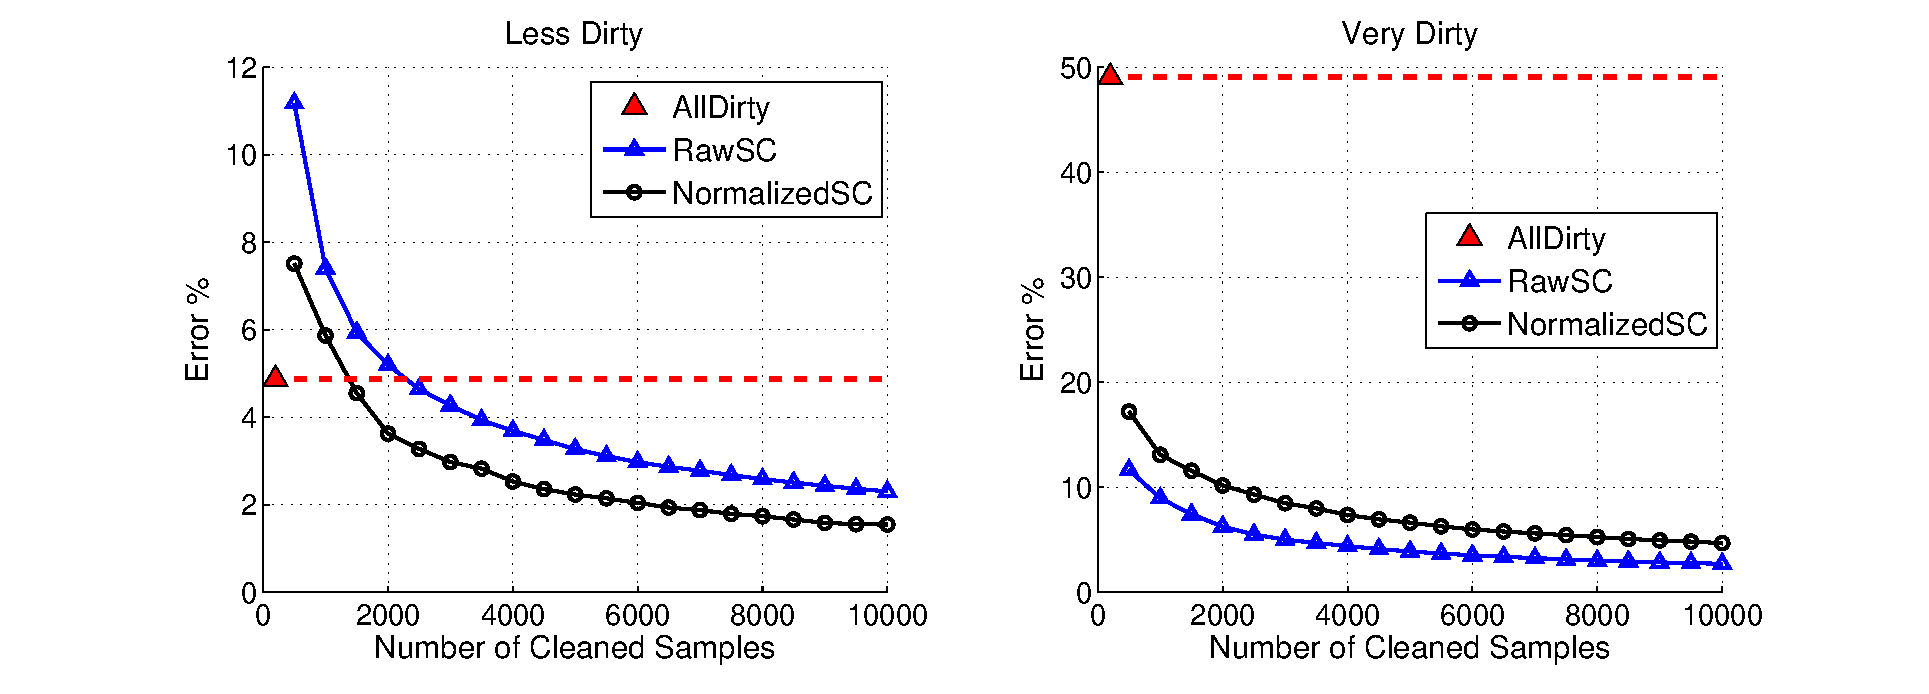
\includegraphics[scale=0.28]{exp/allerror-samplesize.eps}\vspace{-1em}
%\small {\hspace*{2em}(a) High Error Percentage  \hspace{3em} (b) Small Error Percentage}
\caption{Comparison of the convergence of the methods on two TPC-H datasets of 6M tuples with simulated errors (30\% value, 10\% condition, 20 \% duplication) and (3\% value, 1\% condition, 2\% duplication). On the dataset with larger errors, we find that \sampleclean gives a narrower confidence interval, and on the other \biascorrected is more accurate. }\vspace{-1em}
\label{exp:error-samplesize}
%\vspace*{-10pt}
\end{figure}

\subsection{Cleaning Cost v.s. Result Quality}
%One of our key motivations is to find the minimum number of samples to achieve a certain percentage of confidence. 


%\begin{figure}[t]
%\vspace{10pt}
%\includegraphics[scale=0.7]{exp/predicate-samplesize.eps}\\
%\small {\hspace*{2em}(a) 5\% False Positive Errors   \hspace{2em} (b) 50\% False Positive Errors}
%\caption{\sampleclean v.s. BiasCorrect by varying cleaned sample size (False Positive errors = 5\%, 50\%)}
%\label{exp:predicate-samplesize}
%\vspace*{-10pt}
%\end{figure}
%\begin{figure}[t]
%\includegraphics[scale=0.7]{exp/duplication-samplesize.eps}\\
%\small {\hspace*{2em}(a) 5\% Duplication Errors   \hspace{2em} (b) 50\% Duplication Errors}
%\caption{\sampleclean v.s. BiasCorrect by varying cleaned sample size (Duplication errors = 5\%, 50\%)}
%\label{exp:duplication-samplesize}
%\vspace*{-10pt}
%\end{figure}

We evaluated how the number of cleaned samples affects the result error for \sampleclean and \bias.
We ran the \avgfunc query on the two TPC-H datasets that we considered before: one where the percentages for each error type were (30\%,10\%,20\%), and one where each was (3\%,1\%,2\%).
Our results are shown in Figure \ref{exp:error-samplesize}.

Both of the methods converge at a rate $\frac{1}{\sqrt{K}}$ with respect to the sample size.
We can easily estimate how many samples we need to clean to achieve a specified error. %. %\sampleclean performs better on the data with less error while For the data set with more errors,
Another key insight is that since both converge at the same rate with respect to the sample size, the lines will never cross.
Consequently, there will always be a single \emph{better} choice between \sampleclean and \bias, and we do not have to worry about our choice being suboptimal for more cleaned samples.

We also compare our approaches with \alldirty. We can see both \sampleclean and \biascorrected can achieve a better result by cleaning only a small number of samples. Section~\ref{subsec:end-to-end} contains a more detailed comparison with \alldirty and \allclean.
%However, it is important to not the value to which each of these methods converge.
%We can see that \sampleclean and \bias converge to the AllClean value, while SampleDirty converges to the AllDirty value.




\begin{figure*}[t]\vspace{-2em}
\centering
\hspace*{-2em}\includegraphics[scale=0.35]{exp/pk-alldirty-small-errors.eps}\vspace{-1em}
%\small {\hspace*{0em}(a) AVG Query   \hspace{10em} (b) COUNT Query  \hspace{7em} (c) SUM Query}
\caption{TPC-H evaluation with 3\% Value Error, 1\% Condition Error, 2\% Duplication Error on 6M tuples.
Our technique can efficiently estimate on datasets with a small number of errors due to the trade-off between \sampleclean and \bias.}
\label{exp:end-to-end-small}
%\vspace*{-10pt}
\centering\vspace{.5em}
\hspace*{-2em}\includegraphics[scale=0.35]{exp/pk-alldirty.eps}\vspace{-1em}
%\small {\hspace*{0em}(a) AVG Query   \hspace{10em} (b) COUNT Query  \hspace{7em} (c) SUM Query}
\caption{TPC-H evaluation with 30\% Value Error, 10\% Condition Errors, 20\% Duplication Error on 6M tuples.
We find that even for a small number of cleaned samples, we can return results with high confidence.
We are able to achieve 95\% accuracy after cleaning only 0.08\% of the total samples.
%High rates of certain types of random errors, such a duplication, may start to cancel out bias.
%For example, if all of the tuples are duplicated exactly once then there is no need to clean duplicates. 
}
\label{exp:end-to-end}
%\vspace*{-10pt}
\end{figure*}



\subsection{Scalability of Cleaning Cost}

In our \sampleclean and \bias approaches, we return confidence intervals that are independent of the size of the dataset.
In terms of tuples cleaned, there is no difference between evaluating our approach on a 1GB dataset or on a 1TB dataset.
In Figure \ref{exp:scalability-size}, we show that if we simulate the 30\%, 10\%, 20\% errors in different sized TPC-H datasets (1GB, 10GB, 100GB, 1TB) as before, the number of cleaned tuples needed for a certain accuracy remains roughly constant.
Each dataset was generated in the same way; the errors were simulated from the same distribution.
It underscores that the number of samples needed to get a good estimate is a property of the variance of the data and its errors.

\begin{figure}[h]\vspace{-.5em}
\centering
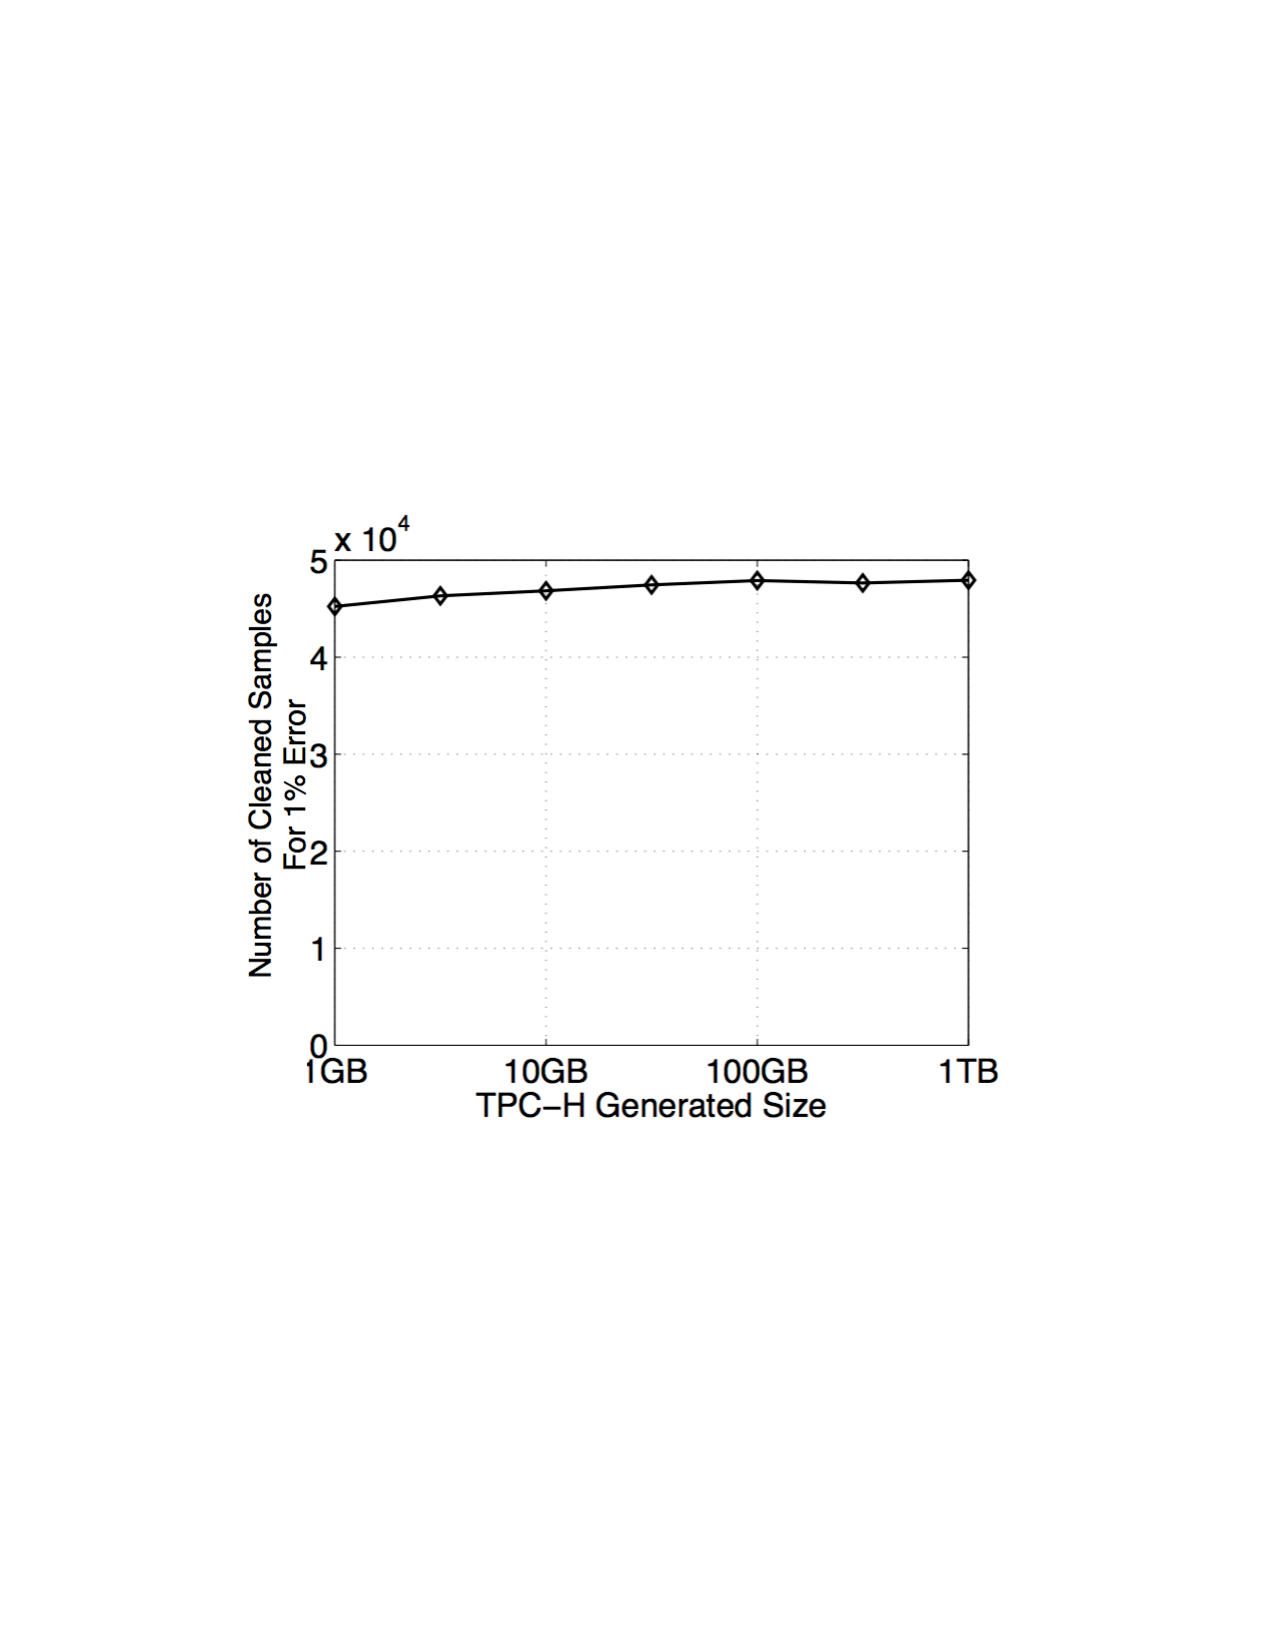
\includegraphics[scale=.4]{exp/scalability-size-cleaning.pdf}\vspace{-1em}
\caption{Scalability of \saqpplus on TPC-H (30\%,10\%,20\%) of different sizes. The number of cleaned tuples needed to achieve a certain accuracy does not increase with the size of the dataset.}\vspace{-.5em}
\label{exp:scalability-size}
%\vspace*{-10pt}
\end{figure}

\begin{figure*}[t]\vspace{-1em}
\centering
\hspace*{-2.5em}\includegraphics[scale=0.31]{exp/imperfect-cleaning-samplesize.eps}\vspace{-1em}
\caption{Imperfect Data Cleaning on TPC-H (30\%, 10\%, 20\%) of 6M tuples. 
Even with a data cleaning technique that is not always correct, we find that our results rapidly converge to the \allclean values.
We found that a 10\% effective cleaning module can give more accurate results than \alldirty with a sample size of 0.03\% of the dataset.}
\label{exp:imperfect}\vspace{-1em}
\end{figure*}



\subsection{End-to-End Experiment}\label{subsec:end-to-end}
We tested the end-to-end performance of the \saqpplus framework on a TPC-H dataset with small errors: 3\% value, 2\% duplication, and 1\% condition errors.
Under these errors, we evaluated the \avgfunc, \sumfunc, and \countfunc aggregations and compared the performance of our framework with \allclean and \alldirty in terms of result quality and cleaning cost.
To process the queries (refer to Section \ref{exp:tpch}), we uniformly sampled from the dataset.
Our results in Figure \ref{exp:end-to-end-small} suggest that \saqpplus quickly converges to the right answer, giving a flexible trade-off between tuples cleaned and the size of the confidence interval in the estimate.
We found that after cleaning only 1000 tuples (0.016\%), we were to estimate more accurately than \alldirty.



This was a dataset with small errors (mostly clean), and we wanted to understand how \saqpplus performs on a much dirtier dataset.
We repeated experiment under 30\% value, 20\% duplication, and 10\% condition errors (Figure~\ref{exp:end-to-end}).
On this dataset \alldirty differs from \allclean by 52\% in the \avgfunc function.
The results in Figure \ref{exp:end-to-end} show that \sampleclean still rapidly converges to the true values and outperforms \alldirty.
In addition, for all queries, our estimate is within 5\% of \allclean after cleaning only 5000 tuples (0.08\% of the total data).

Due to the trade-off between \bias and \sampleclean, we can estimate accurately for datasets that are both mostly clean or very dirty.
On the dataset with small errors, \bias was the more accurate estimation method and \sampleclean was more accurate on one in the presence of larger errors.
%Our technique is scalable since for both \sampleclean and \bias,
%we return confidence intervals that are independent of the size of the dataset.
%These confidence intervals are only dependent on the size of the sample, and the variance of the data.
%The number of samples needed to get a good estimate is really a property of the data and its errors, and not the size of the dataset.


\begin{figure*}[t]\vspace{-2.5em}
\hspace*{-2em}
\includegraphics[scale=0.35]{exp/msacademic-paper-count.eps}\vspace{-1em}
\caption{The output of our result estimation framework for each author. The dataset was particularly dirty and cleaning only 50 tuples per author was sufficient to outperform an aggregation of the entire dataset.}
\label{exp:ms-academic-paper-count}
\end{figure*}

\subsection{Imperfect Data Cleaning}
\label{exp:sensitivity}

%Our approach is general enough to incorporate data cleaning that is imperfect (an \allclean result does not correspond to a true value).
%The confidence intervals we provide are with respect to \allclean and not dependent on knowing the true values.
In Figure \ref{exp:imperfect}, we experimentally show that \saqpplus is valuable even when the cleaning is incomplete.
We ran our experiments on a dataset with 30\% Value Errors, 10\% Condition Errors, and 20\% Duplication Errors, and simulated
a data cleaning technique that can only identify and clean a fixed percentage of errors.
We compared the Error \% of the query and the total sample size including tuples where the data cleaning failed.

Even though our estimates are now biased with respect to the true values, they are still unbiased with respect to \allclean.
Consequently, we found that even if our cleaning technique can clean only 10\% of the errors, we still only have to sample 2,000 tuples to achieve a more accurate result than \alldirty.
Furthermore, we can take advantage of both \sampleclean and \biascorrected.
If a technique changes a lot of the tuple values, then \sampleclean gives us a more precise estimate.
However, if a technique keeps most of the values the same \biascorrected is more precise.




\begin{figure}[t]\vspace{-1.8em}
\centering
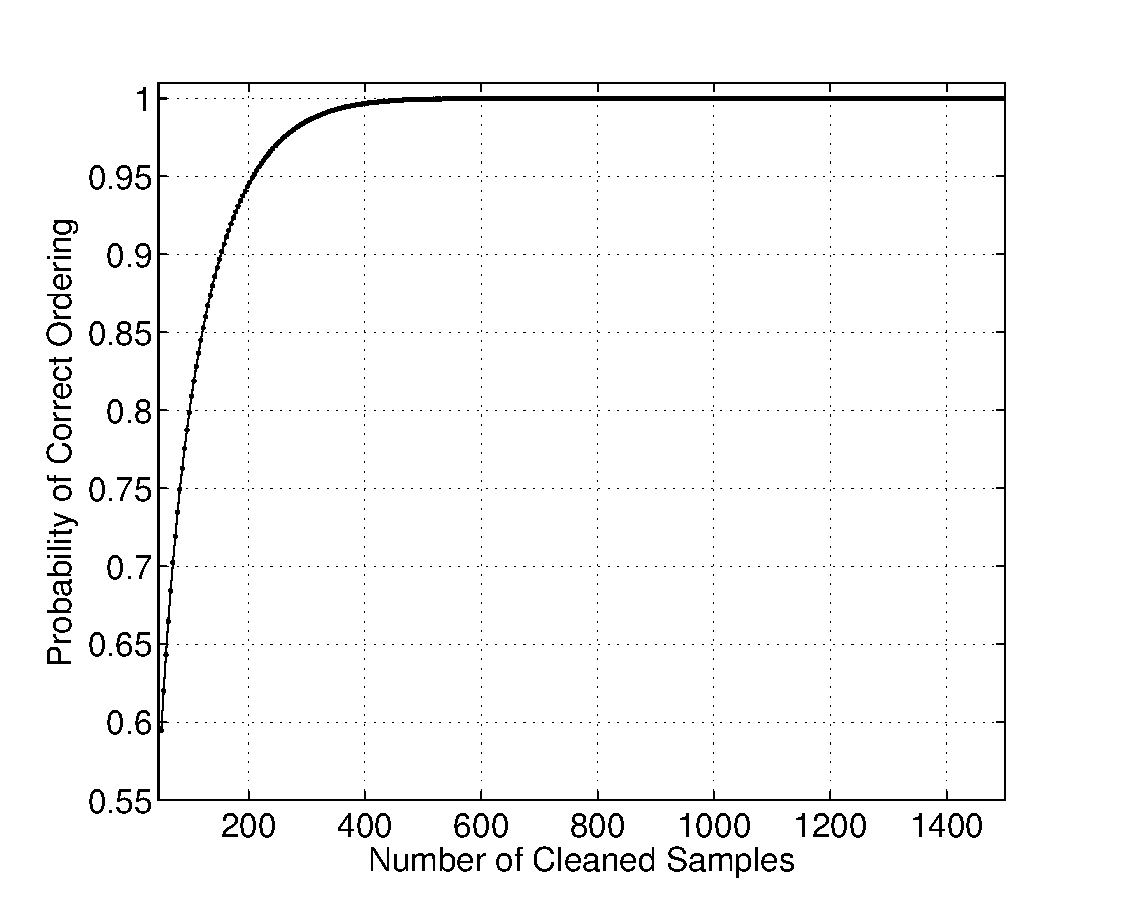
\includegraphics[scale=0.3]{exp/msacademic-paper-ranking.eps}
\caption{Even though \alldirty always returns an incorrect ranking, we can return the correct ranking with 95\% probability after cleaning only 210 total samples. To achieve a correct ranking with 99\% probability, we require 326 samples to be cleaned.}\vspace{-1em}
\label{exp:ms-academic-ranking}
\end{figure}

\subsection{Evaluation on Real Data}
The following sections contain experiments on two real datasets: Microsoft Academic Search and the Intel Lab Sensors.
As described in Section~\ref{subsec:dateset}, they contain different types of errors: the sensor dataset consists of predominantly value and condition errors, and the publication dataset consists of condition and duplication errors.

\subsubsection{Microsoft Academic Search}\label{exp:mas}
We designed this experiment to be illustrative of assessing the confidence of decisions based on dirty data, by trying to get an accurate publication count for the 
three authors.
We can see that in Table~\ref{tbl:dataset:ms-academic} AllDirty not only returns incorrect values but also returns an incorrect ranking of the three authors.
This is an example of a dataset where the data cleaning is quite well defined, we can apply our domain expertise in database publications to reason about each tuple in the dataset, but cleaning is very time consuming. 
In Figure \ref{exp:ms-academic-paper-count}, we show how our approach can budget data cleaning for each author up-to a desired query quality.
We clearly see that our estimates are centered around the AllClean value and even with the confidence intervals outperform aggregations of the full dirty data.

However, we do notice that the confidence intervals for the estimated paper counts overlap for a small number of cleaned samples.
We evaluated how many tuples would need to be cleaned to get an accurate ranking using a simulation; that is if we re-ran the same experiment with the same sample size what is the probability our ordering of the authors is accurate.
For each author, we treat the estimate of their paper count as a normally distributed random variable.
From these distributions, we sample 10000 paper counts and calculate the empirical probability of an incorrect ordering.
In Figure \ref{exp:ms-academic-ranking}, we show how we can return the correct ranking with 95\% probability after cleaning only 210 total samples.
To achieve a correct ranking with 99\% probability, we require 326 samples to be cleaned.
In comparison, AllDirty always returns an incorrect ranking.
\saqpplus provides a flexible way to achieve a desired confidence on decision based on dirty data queries.



\subsubsection{Sensor Dataset}
\begin{figure*}[t]\vspace{-2.5em}
\hspace{-60pt}
\includegraphics[scale=0.375]{exp/sensor-all-queries.eps}\vspace{-1em}
\caption{Queries applied to the sensor dataset. We applied a set of queries with a fixed sample (same for all queries) of 500 cleaned tuples. We compare the error percentage (log-scale) of AllDirty, \sampleclean, and \bias with respect to AllClean.
 For all of these example queries, we are able to achieve a relative error of less than $\pm 10\%$ even when the data error is orders of magnitude higher.}\vspace{-1em}
\label{exp:sensor-all-queries}
\end{figure*}
The sensor dataset consists of readings from inexpensive battery-operated sensors.
The failure mode of these sensors is returning incorrect readings, particularly when the available battery power is low.
We limited the dataset to a single month where the readings from the beginning of the month were largely accurate, while the readings from later in the month became increasingly inaccurate.
We cleaned 500 samples (1.12\%) of the dataset using the algorithm described in~\cite{DBLP:conf/pervasive/JefferyAFHW06} and applied a variety of queries to illustrate how different types of value and condition errors can affect results (Figure \ref{exp:sensor-all-queries}).

Like the TCP-H results, this experiment shows how having both \sampleclean and \bias helps us estimate accurately in different error distributions.
Surprisingly, we found that different queries on the same dataset may have very different error characteristics making the choice between \sampleclean and BiasCorrect very important.
From this experiment, we can also see the interactive latency capabilities of \saqpplus.
Since we cleaned the 500 sampled tuples, subsequent \sampleclean queries only need to operate on the cleaned sample.
This demonstrates how \sampleclean can give a very fast response time on large datasets as it only has to process the tuples in the cleaned sample.

The first two queries \texttt{avg}(temp) and \texttt{avg}(light) illustrate the severity of the sensor errors.
Simply taking an average over the dirty data results in an estimate that differs from AllClean by about 100\%.
However, for the cost of cleaning only 500 samples, we are able to achieve a confidence interval of $\pm 1.5\%$ and $\pm 15.2\%$ respectively.
Due to the nature of the sensor errors, a similar, but more dramatic, improvement is seen for \texttt{var}(temp) and \texttt{var}(light).
Random errors such as ones generated by electronic sensors tend to increase variance of the data, and we can see that our estimate for \texttt{var}(temp) is three orders of magnitude closer to AllClean.

We also evaluated the queries with predicates.
In the first query, we looked at the average temperature when the humidity was above 30\%.
For this query, there were both value and condition errors.
We also looked at the average temperature when the predicate attribute (time) was accurate even during sensor failures.
We found that our technique works well in both cases giving significant improvements over aggregations of the dirty data.

Finally, we demonstrate a query where the errors are relatively small.
We counted the number of readings where the temperature was above some threshold.
We found that the dirty aggregation was not very much worse than the confidence intervals returned by our method.
Furthermore, we also experimented with the average temperature over the first four days when most of the sensors were working.
In this query, AllDirty differed from AllClean by less than 1\%. 
In fact, AllDirty outperforms \sampleclean for 500 cleaned samples.
However, due to our tradeoff between \sampleclean and \bias, we are still able to improve on already good estimates.

%\subsubsection{MSAcademic/GoogleScholar Dataset}

%\begin{table*}[ht]
%\tiny
%\caption{For each example query we simulated the benefit of cleaning the MSAcademic/GoogleScholar Dataset. We report the Data Error, and the number of samples that need to be cleaned to achieve an 25\%, 50\%, and 75\% reduction in this error.}
%\label{exp:citations}
%\centering 
%\begin{tabular}{c c c c c c}
%\hline\hline
%No. & Query & Dirty Data Error & +25\% acc. &+50\% acc. & +75\%acc. \\ 
%\hline  % inserts single horizontal line
%1 & SELECT \textsf{AVG}(citation) FROM publication& 71.03\% & 28 & 105 & 577 \\
%2 & SELECT \textsf{SUM}(citation) FROM publication& 71.03\% & 28 & 105 & 577 \\ 
%3 & SELECT \textsf{COUNT}(citation) FROM publication& 3.96\% & 85 & 186 & 585 \\
%\hline  % inserts single horizontal line
%4 & SELECT \textsf{COUNT}(citation) FROM publication WHERE citation $\ge$ 50 & 56.35\% & 37 & 90 & 341 \\
%5 & SELECT \textsf{AVG}(citation) FROM publication WHERE citation $\ge$ 50 & 48.65\% & 370 & 723 & 1441 \\
%6 & SELECT \textsf{COUNT}(citation) FROM publication WHERE citation == 0 & 71.84\% & 132 & 283 & 811 \\
%\hline  % inserts single horizontal line
%7 & SELECT \textsf{COUNT}(citation) FROM publication WHERE year > 1980 & 3.55\% & 153 & 302 & 945\\
%8 & SELECT \textsf{COUNT}(citation) FROM publication WHERE year > 1980 *& 3.55\% & 1450 & 1725 & 2000\\
%9 & SELECT \textsf{AVG}(citation/(2013-year)) FROM publication & 69.31\% & 34 & 76 & 381\\
%\hline %inserts single line
%\end{tabular}
%\end{table*}

%We applied our framework on this dataset of paper citations.
%The experiment considers the data as a single table \textbf{publication} with the attributes \textbf{citation} (number of citations received by the paper) and \textbf{year} (the year of publication).
%We assume that there are only errors in the \textbf{citation} attribute.
%We present a set of 9 example queries and their results (Table \ref{exp:citations}).
%For each query, we evaluated what the uncleaned result would be, then calculated the number of clean samples needed to out perform a dirty aggregation by 25\%, 50\%, and 75\%.

%Our results illustrate that a naive aggregation of the dirty data (eg. Query 1) could result in an estimate is more than 70\% away from the true value.
%If we take the Query 1 as an example, even for a relatively small number of cleaned tuples (about 5\% of the data) we can reduce this error by 50\%.

%It is important to note the errors in this dataset are not independently random errors.
%We can see indications of strong systemic error in comparing the quality of Query 3 and Query 4.
%It is clear that papers with a larger number of citations were more likely to be duplicated.
%In addition, we see that there is a complex dependency of the quality of an estimate and the data and error variance.
%If we compare Query 4 and Query 5, we see that the simple change of aggregation function requires much more cleaning for similar accuracy.

%We can also experiment with more complex multi-attribute queries.
%In Query 7 and Query 8, we illustrate a point about dealing with combinations of errors and best practices when executing these queries.
%Query 7 counts the number of papers in the dataset published after 1980, and not surprisingly the results are similar to that of Query 1; where the only source of error is a small duplication error.
%However, Query 8 executes the same count in a different way.
%If we treat the entire set of papers as our population, and mark those that were published before 1980 as false positives we can still get an unbiased estimate.
%However, setting many elements to zero in $\phi_f(.)$ increases the variance of the estimate and we require many more cleaned tuples to answer the same query.
%This is related to the point made in Section \ref{sec:optimization}, where we skip false positives in the mean query to reduce estimate variance.

%Finally, we demonstrate the performance on a multi-dimensional query.
%Query 9 calculates the average number of citations per year received by the papers in the dataset.

%\subsubsection{GoogleScholar Author Profile}
%\begin{figure}[t]
%\centering
%\hspace*{-2em}\includegraphics[scale=0.45]{exp/false-positive-error-weiwang.eps}\\
%\caption{We estimated the total number of citations for confirmed publications on the dirty dataset from the author's GoogleScholar Author Profile. We were unable to confirm over 95\% of the publications, and treated those as false positive errors.}
%\label{exp:wei-wang-fp}
%\vspace*{-10pt}
%\end{figure}
%Given this profile dataset with a very high false positive rate, we tried to estimate the total number of citations received by the author.
%The sum over all the confirmed publications is 5735 citations, while over the entire dataset it is 13108.
%Our results in Figure \ref{exp:wei-wang-fp}, show that we easily outperform an aggregation of the full dirty data.
%For even 50 cleaned samples our error bound is less than the data error.

%However, if we measure error with respect to the true value we do require a lot more cleaning.
%For example, if we want to get within 10\% of the true value, we require 1406 sample cleaned.
%With a 95\% false positive error, this is an inherently hard dataset to estimate, and as a result we have to clean a large number of samples to get accurate estimates.

%\subsubsection{Entity Resolution Datasets}
%\begin{figure*}[t]
%\centering
%\hspace*{-5em}\includegraphics[scale=0.40]{exp/entity-resolution.eps}\\
%\small {\hspace*{1em}(a)Papers \hspace{11em} (b)Restaurants  \hspace{11em} (c)Products}
%\caption{We evaluate the \textbf{COUNT} query on three datasets with duplication errors. Our results show that even for a small sample of cleaned data tuples
%our estimates are relatively close to the true value.}
%\label{exp:entity-res}
%\vspace*{-10pt}
%\end{figure*}

%We applied our framework to the three entity resolution datasets to answer a count of the number of distinct elements (Figure \ref{exp:entity-res}).
%The results suggest good estimates on datasets with large number of duplicates as well as ones with a relatively small number of duplicates.
%It is interesting to note that we see that even sampling 100 or 200 clean tuples can result in a much better estimate than an exact aggregation of the dirty data.
%Another interesting point is in datasets such as the product dataset, where almost every tuple has 1 duplicate, the sample variance of our transformed data sequence
%is small resulting in very accurate estimates.
%This illustrates a key point that small duplication errors may be harder to handle than large number of duplicates.
%\reminder{Use my gnuplot template, and change the starting value of the y-axis to zero for each subfigure.}

%\subsection{Group By and Constrained Queries}
%\begin{figure}[t]
%\centering
%\hspace*{-2em}\includegraphics[scale=0.36]{exp/groupby-constraints.eps}\\
%\small {(a)500 tuples cleaned (b)1000 tuples cleaned}
%\caption{We calculated the mean citations for papers written in each decade, subject to cleaning constraints. Our estimates and confidence intervals are closer to the true value than an aggregation of the entire dirty data.}
%\label{exp:groupby-constraints}
%\vspace*{-10pt}
%\end{figure}
%We evaluated our query processing framework with \textbf{group by} queries with cost constraints on the MS Academic-Google Scholar Dataset.
%We ran the following two queries to calculate the mean number of citations per paper in each decade:
%\begin{alltt}
%SELECT \textsf{AVG}(CITATIONS) FROM Publication
%WHERE Conference = "\textsf{SIGMOD}"
%GROUP BY round(Year/10)
%WITHIN COST 500 TUPLES
%\end{alltt}

%\begin{alltt}
%SELECT \textsf{AVG}(CITATIONS) FROM Publication
%WHERE Conference = "\textsf{SIGMOD}"
%GROUP BY round(Year/10)
%WITHIN COST 1000 TUPLES
%\end{alltt}

%The results are shown in Figure \ref{exp:groupby-constraints}, and we can clearly see that the estimates and the confidence intervals outperform an aggregation of the entire dirty data.
%We can also see that increasing the budget reduces the maximum error by targeting the populations that have the biggest uncertainty.
%An important point is that the allocation algorithm is relatively sensitive to the initial estimates of variance.
%If we don't clean a sufficiently large constant sample of data to get an initial estimate of the error for each population, then the algorithm could give an allocation that is far from optimal.


\vspace{-1em}
\section{Related Work}\label{sec:rw}
{\noindent \bf Approximate Query Processing:} \saqp has been studied for more than two decades~\cite{DBLP:conf/vldb/GarofalakisG01,DBLP:journals/ftdb/CormodeGHJ12}.
Many \saqp approaches~\cite{DBLP:journals/tods/ChaudhuriDN07,DBLP:conf/eurosys/AgarwalMPMMS13,DBLP:conf/sigmod/AcharyaGPR99,DBLP:conf/cidr/SidirourgosKB11,DBLP:conf/sigmod/BabcockCD03,DBLP:conf/sigmod/HellersteinHW97,DBLP:journals/pvldb/PansareBJC11,DBLP:conf/sigmod/CondieCAHGTES10,DBLP:journals/pvldb/WuJOT09} were proposed, aiming to enable interactive query response times.
%Acharya et al.~\cite{DBLP:conf/sigmod/AcharyaGPR99} developed the Aqua system which is run on top of relational DBMS, and allows users to obtain approximate query answers in a fast response time. Chaudhuri et al.~\cite{DBLP:journals/tods/ChaudhuriDN07} studied how to create an optimal stratified random sample based on a given query workload, and proposed the STRAT algorithm that can make the workload queries achieve the best quality on the sample. Sidirourgos et al.~\cite{DBLP:conf/cidr/SidirourgosKB11} presented the SciBORQ architecture that creates biased multi-layered samples based on the scientific data exploration workload, and adaptively select a suitable sample to satisfy quality or time constraints during query execution. Agarwal et al.~\cite{DBLP:conf/eurosys/AgarwalMPMMS13} devised novel multi-dimensional stratified samples based on real-world big data analytics workloads, and built the BlinkDB system to utilize the created samples to support interactive query processing with error and response time constraints. Unlike the above approaches which create samples ahead of query time, online aggregation~\cite{DBLP:conf/sigmod/HellersteinHW97,DBLP:journals/pvldb/PansareBJC11,DBLP:conf/sigmod/CondieCAHGTES10,DBLP:journals/pvldb/WuJOT09} constructs samples in an online fashion, and gradually achieve more and more accurate results until users are satisfied about the current results. 
There are also many studies on creating other synopsis of the data, such as histograms or wavelets~\cite{DBLP:journals/ftdb/CormodeGHJ12}. While a substantial works on approximate query processing, these works mainly focus on how to deal with sampling errors, with little attention to data errors. 

\vspace{.5em}

{\noindent \bf Data Cleaning:} There have been many studies on various data-cleaning techniques, such as rule-based approaches~\cite{fan2012foundations,DBLP:conf/sigmod/DallachiesaEEEIOT13}, outlier detection~\cite{hellerstein2008quantitative,dasu2003exploratory}, filling missing values~\cite{conf/icde/BethTMP13, parkcrowdfill}, and duplicate detection~\cite{conf/hdkm/Christen08, DBLP:conf/kdd/BilenkoM03, conf/sigmod/WangLF12}. In order to ensure reliable cleaning results, most of these techniques require human involvement~\cite{DBLP:conf/sigmod/JefferyFH08,DBLP:journals/pvldb/FanLMTY10,DBLP:journals/pvldb/YakoutENOI11,DBLP:journals/pvldb/WangKFF12,DBLP:conf/sigmod/WangLKFF13}. 
%For example, Fan et al.~\cite{DBLP:journals/pvldb/FanLMTY10} proposed to employ editing rules, master data and user confirmation to clean data, and proved that their approaches can always lead to correct cleaning results. Wang et al.~\cite{DBLP:journals/pvldb/WangKFF12} proposed a hybrid human-machine approach to detect duplicate entities in data, which can achieve higher detection accuracy than machine-only approaches. 
In our paper, the main focus is not on a specific data-cleaning technique, but rather on a new framework that enables a flexible trade-off between data cleaning cost and result quality.
Indeed, we can apply any data-cleaning technique to clean the sample data, and then utilize our framework to estimate query results based on the cleaned sample. 


\vspace{.5em}

{\noindent \bf Result Estimation and Sampling:}
Estimating aggregate statistics of populations from samples has been well studied in the field of surveying \cite{weisberg2009total,valliant2000finite, hansen1987some, barnett1991sample, sarndal2003model, kalton1983introduction}.
These works explore different types of sampling, error characterizations, bias-variance trade-offs, and confidence intervals.
The theoretical foundation of surveying is statistical bounding of functions of independent random variables (e.g., samples with replacement).
This field includes distribution-free bounds such as Markov/Chebyshev/Hoeffding bounds, asymptotic bounds such as the Central Limit Theorem (CLT), and empirical testing such as Bootstrapping \cite{hinkley1988bootstrap}.
For a detailed survey of different types of statistical bounds refer to \cite{hahn2011statistical}.
Due to the CLT's strong guarantees (unbiased sample estimates and normalcy), as in our work, it is widely applied in the analysis of sampling schemes.
The more general study of sample estimators that are unbiased and have asymptotically normal distributions (like the CLT) is called U-Statistics, refer to \cite{lee1990u} for a survey of this theory.
The stochastic process literature also discusses problems in unbiased estimation from samples \cite{jacod1987limit}.

\vspace{.5em}

{\noindent \bf Distinct Value Estimation:}
Distinct value estimation has been an open problem in stream processing and database research~\cite{considine2004approximate,bar2002counting,haas1995sampling,beyer2007synopses}.
Similar to our analysis, some have argued that simply removing duplicates in a sample of data does not work~\cite{charikar2000towards}.
In the storage literature, similar weighted average techniques have been applied for global file duplication rate estimation \cite{harnik2012estimation} based on the knowledge of duplication rates within a sample.
This work can be seen as a simplified version of our problem only answering a count query with only duplication errors.
Techniques similar to our duplicate reweighting scheme have been studied in estimating from non-uniform samples \cite{aldroubi2002non}, and is also similar to the acceptance ratio used sampling algorithms such as the Metropolis-Hastings Algorithm and Rejection Sampling \cite{liu1996metropolized,metropolis1953equation}.
Further relevant work includes sensitivity analysis of set functions \cite{mcdiarmid1989method, jukna2012analysis} and statistical information theory \cite{kullback1997information}. 


\vspace{-.5em}
\section{Conclusion and Future Work}\label{sec:con}
In this paper, we explore using sampling, integrated with data cleaning, to improve answer quality. We propose \saqpplus, a novel framework which only requires users to clean a sample of data, and utilizes the cleaned sample to obtain unbiased query results with confidence intervals.
We identify three types of data errors (i.e., value error, condition error and duplication error) that may affect query results, and develop \biascorrected and \sampleclean to estimate query results for the data with these errors.
Our analysis and experiments suggest that \saqpplus, which returns the better result between \biascorrected and \sampleclean, is robust to different magnitudes and rates of data errors, and consistently reports good estimate results.
%Moreover, \saqpplus can optimally satisfy user-specified cleaning-cost or result-quality constraints.
Our experiments on both real and synthetic data sets indicate that \saqpplus only needs to clean a small sample of the data to achieve accurate results, and furthermore the size of this sample is independent of the size of the dataset.
In particular, \sampleclean, which processes queries only on the cleaned sample, not only makes the query processing more scalable, but surprisingly may provide higher quality results than an aggregation of the entire dirty data (\alldirty).

To the best of our knowledge, this is the first work to marry data cleaning with sampling-based query processing.
%But, it is merely the tip of the iceberg.
There are many research directions for future exploration. 

\vspace{.25em}
{\noindent \bf Constrained Queries:} Now that we have quantified a tradeoff between cleaning costs and result quality, we can explore query results where users can specify a cost or quality constraint. For example, users may want to know that given a cleaning budget, what is the best result quality they can achieve? Or, given a quality constraint, how many samples they need clean to meet the constraint? 
In these constrained queries, we aim to answer with an optimal cost or most accurate result to meet the constraints.

\vspace{.25em}
{\noindent \bf Uncertain Cleaning Results:}  Our framework can return unbiased query results with respect to AllClean for a variety of different data cleaning approaches.
We are also interested in how we can incorporate uncertain or probabilistic cleaning processes into this framework.
For example, given a dirty record, could the data cleaning module specify a set of ranges for each attribute? 
We are interested in what guarantees, if any, we can achieve in such settings.

\vspace{.25em}
{\noindent \bf Complex SQL Queries:} Another important avenue of future work is to extend our framework to support more complex SQL queries such as join and nested SQL queries. There are some straightforward methods to implement these queries. For example, we can materialize the join result as a single table, and then apply our framework to the materialized table. But this could be very costly for large datasets, thus we need to explore more efficient implementations.
For a larger set of queries, it may not be possible to estimate their results with the CLT.
Thus, exploring empirical estimation approaches (such as bootstrapping) to our framework is another interesting future direction.

\vspace{.25em}
{\noindent \bf Sample Maintenance:} Finally, in real applications users may create multiple samples from the data.
Maintaining these samples for data updates is also very challenging and needs to be investigated.


\vspace{1.5em}

\fussy
{\noindent  \bf Acknowledgements.} {\small  The authors would like to thank Sameer Agarwal, Bill Zhao, and the SIGMOD reviewers for their insightful feedback. This research is supported in part by NSF CISE Expeditions Award CCF-1139158, LBNL Award 7076018, DARPA XData Award FA8750-12-2-0331, the European Research Council under the FP7, ERC MoDaS, agreement 291071, and by the Israel Ministry of Science, and gifts from Amazon Web Services, Google, SAP, The Thomas and Stacey Siebel Foundation, Apple, Inc., Cisco, Cloudera, EMC, Ericsson, Facebook, GameOnTalis, Guavus, Hortonworks, Huawei, Intel, Microsoft, NetApp, Pivotal, Samsung, Splunk, Virdata, VMware, WANdisco and Yahoo!.
}
\sloppy





{
\bibliographystyle{abbrv}
%\fontsize{7pt}{7.9pt} \selectfont
\scriptsize
\bibliography{refs/crowdsourcing,refs/bigdata,refs/er,refs/stats}
}

\clearpage
\newpage
\section{Appendix}
The appendix is organized in the following way.
In Section \ref{app:proof}, we prove the unbiasedness of our estimation.
In Section \ref{app:ext}, we discuss how \sampleclean and \bias can be extended to different functions, including \varfunc.
Finally in Section \ref{app:ext2}, we discuss how \bias can be extended to make unbiased estimates from existing sample aggregations.

\subsection{Proofs}\label{app:proof}
In this section, we detail the theorems and the lemmas used in the paper.
Our main goal is to show that our estimates are unbiased; that is in expectation (denoted by $\mathbb{E(.)}$) they give the right answer.
Throughout these proofs, we will apply some key properties of expected values, for random variables $x$ and $y$:
\begin{itemize}
\item Linearity: $\mathbb{E}(ax+by)=a\mathbb{E}(x)+b\mathbb{E}(y)$
\item Independence: if $x$ and $y$ are independent then \\$\mathbb{E}(f(x)g(y))=\mathbb{E}(f(x))\mathbb{E}(g(y))$
\item Measurable functions: $\mathbb{E}(f(x))= \int f(x) \mathbb{P}(x)$ or in the discrete case $\mathbb{E}(f(x))= \sum f(x) \mathbb{P}(x)$
\end{itemize}

\subsubsection{Unbiased Estimates From Reweighted Data}
We proposed a reweighting technique to account for the over-representation of duplicates in samples.
To show that this gives us an unbiased estimate, our proof strategy will be to prove results on the full dataset, and then extend the results to a sample.

{\noindent \bf \avgfunc query:}
We begin with the following basic lemma about reweighting the entire dataset and how a mean of the reweighted data differs from the true mean.

\setcounter{lemma}{0}
\begin{lemma}
Let $P$ be a population with $N$ data tuples, and $P_{u}$ be the cleaned population with $N'$ unique data tuples.
For each $p_{i}\in P$, let $m_i$ denote the number of its duplicates in $P$.
Then mean value of the set $\saqpplusfunc(P)=\{\frac{p_{1}}{m_{1}},\frac{p_{2}}{m_{2}},...,\frac{p_{N}}{m_{N}}\}$ is:
\[
mean(\frac{N}{N'}\saqpplusfunc(P))= mean(\hat{P}_{u})
\]
\end{lemma}

Proof: The function $\saqpplusfunc$ acts point-wise on the elements of the dirty set $P$, creating a new set $\saqpplusfunc(P)$.
Therefore:
\[
mean(\saqpplusfunc(P)) = \frac{1}{N}\sum_i^N \frac{x_i}{m_i}
\]
We collect all the terms with the same value; that is a set ${i:x_i=z}$.
We call the set of distinct values the support, denoted by $supp(p)$.
\[
mean(\saqpplusfunc(P)) = \frac{1}{N}\sum_{z \in supp(p)} z(\sum_i \frac{1}{m_i})
\]
If we mutliply each $z$ by $\frac{N'}{N}$, then:
\[
mean(\saqpplusfunc(P)) = \sum_{z \in supp(p)} z\frac{(\sum_i \frac{1}{m_i})}{N'}
\]

The aggregation attributes of a population of numerical tuples can be interpreted as a discrete probability distribution.
For example, in the set $\{1, 1, 3\}$, we can say that an equivalent representation is a distribution $p(x)$, where $p(1)=\frac{2}{3}$,
and $p(3)=\frac{1}{3}$.
This probability distribution is exactly the probablity that a value will be drawn in a uniform random sampling.
Furthermore, let us say that $p(x)$ is a representation for the clean population $P_{u}$.
The expected value of this distribution is consistent with the mean of the set:
\[
\mathbb{E}(p(x)) = \sum_z z \mathbb{P}(x=z)
\]
\[
\mathbb{E}(p(x)) = mean(P_{u})
\]
and furthermore $\mathbb{P}(x=z)=\frac{(\sum_i \frac{1}{m_i})}{N'}$:
\[
mean(\frac{N}{N'}\saqpplusfunc(P))= mean(\hat{P}_{u})\blacksquare
\]

We use this lemma to prove that our estimates on a sample are unbiased.
This was presented as Lemma \ref{lem:derror} in paper.
Specifically, we mean that in expectation the mean of $\saqpplusfunc(S)$ is equal to result on the full cleaned data $\saqpplusfunc(P)$.
\begin{lemma}
Let $S \subseteq P$ be a sample of a population with $K$ data tuples, and $P_{u}$ be the cleaned population as defined before.
For each $s_{i}\in S$, let $m_i$ denote the number of its duplicates in $P$.
Then expected mean value of the set $\saqpplusfunc(S)=\{\frac{s_{1}}{m_{1}},\frac{s_{2}}{m_{2}},...,\frac{s_{K}}{m_{K}}\}$ is:
\[
\mathbb{E}(\frac{K}{K'}mean(\saqpplusfunc(S))) = mean(P_{u})
\]
where $K'=\sum_i\frac{1}{m_i}$.
\end{lemma}
Proof: A caveat is that $m_i$ is also a random variable.
Since, we assume uniform random sampling, we can conclude that each $s_i,m_i$ are independent from other samples:
\[
s_{i} \perp s{j}\text{, } m_{i} \perp m{j}
\]
Using this intuition, we want to isolate a sample and its duplication number.
Let us first consider a single sample $s_{i}$ from the mean calculation,
we hold out the terms relating to $i$ and express it as:
\[
\frac{K}{\frac{1}{m_i}+ \sum_{j\ne i}\frac{1}{m_j}} \frac{s_i}{m_i}
\]
With a little bit of algebraic manipulation, we can get:
\[
\frac{K(\sum_{j\ne i}\frac{1}{m_j})}{(K-1)\sum_i\frac{1}{m_i}}\cdot\frac{K-1}{\sum_{j\ne i}\frac{1}{m_j}}\cdot\frac{s_i}{m_i}
\]
Now, if we take expectations,
\[
\mathbb{E}(\frac{K(\sum_{j\ne i}\frac{1}{m_j})}{(K-1)\sum_i\frac{1}{m_i}}\frac{K-1}{\sum_{j\ne i}\frac{1}{m_j}}\frac{s_i}{m_i})
\]
apply linearity, and notice the symmetry in the problem (if we sample independently each samples is probabilistically the ``same");
we can see that by the first term will be 1 in expectation.
In other words, since we are holding out 1 item each time, which means the average will be exactly $\frac{K}{K-1}$.
We are left with:
\[
\mathbb{E}(\frac{K-1}{\sum_{j\ne i}\frac{1}{m_j}}\frac{s_i}{m_i})
\]
Applying independence to the rest of the expression, this is equal to:
\[
\mathbb{E}(\frac{K-1}{\sum_{j\ne i}\frac{1}{m_j}})\mathbb{E}(\frac{s_i}{m_i})
\]
The first term in an independent unbiased estimate of $\frac{N}{N'}$ and the second term is mean of $mean(\saqpplusfunc(P))$:
\[
\frac{N}{N'}\cdot mean(\saqpplusfunc(P)) = mean(P_{u})\blacksquare
\]

{\noindent \bf \sumfunc and \countfunc queries:}
These queries follow from the same logic as the \avgfunc query, but with a much simplified proof for both lemmas.
As we do not need to deal with a scaling factor such as $\frac{N}{N'}$, the first theorem is trivially shown by linearity of expectation.
In the second theorem, since we can treat $\frac{s_i}{m_i}$ as a single random variable (there is no dependence of $K'$ on $m_i$) so each sample
is trivially independent.
We can then use the fact that sample means are unbiased estimators of population means.

\subsubsection{Unbiased Estimates With Predicates}\label{app:proof2}
A similar proof is needed to show that estimates with predicates are unbiased.

{\noindent \bf \avgfunc queries:}
We will explore how predicates affect the \avgfunc query.
\begin{lemma}
Let $S \subseteq P$ be a sample of a population with $K$ data tuples, and $P_{1}\subset P$ be the set of tuples that satisfy the predicate.
For each $s_{j}\in S$, let $I(j)$ be an indicator function of whether the tuple satisfies the predicate or not.
Then expected mean value of the set $\saqpplusfunc(S)=\{I(1)s_1,I(2)s_2,...,I(K)s_K \}$ is:
\[
\mathbb{E}(\frac{1}{r}mean(\saqpplusfunc(S)))= mean(P_{1})
\]
where $r = \frac{\sum_j I(j)}{K}$.
\end{lemma}
Proof: We first can expand the expression, noticing that the factors of $K$ cancel out:
\[\frac{1}{r}mean(\saqpplusfunc(S)) = \frac{1}{\sum_j I(j)}\sum_n I(n)s_n \]
Since only the non-zero elements contribute to the sum, then this is the same as the mean over the elements in
the sample that satisfy the predicate.
Then, it follows that, in expectation, each sample that satisfies the predicate has mean:
\[ mean(P_{1})\]
Applying the linearity of expectation:
\[
\mathbb{E}(\frac{1}{r}mean(\saqpplusfunc(S)))= mean(P_{1})\blacksquare
\]

{\noindent \bf \sumfunc and \countfunc queries:}
Similar to duplication error, as we do not have to worry about the scaling factor $r$ for these quries the proof is greatly simplified.
In fact, as before it directly follows from the linearity of expectation.



\subsubsection{Proof of Theorem~\ref{thm:sampleclean}}\label{app:proof3}
The lemmas in the previous sections for duplication errors and predicates are careful to prove unbiased estimates only under their respective errors.
However, the theorems are general enough not to make any assumptions about the presence of other errors.
We can compose these corrections in the intuitive way; where we first set the attribute to its correct value, reweight the value by $m_i$, and set it to $0$ if it does not satisfy the predicate.

The proof is clear, since we are taking one pass making the estimate unbiased under value errors.
Then in another pass our estimate is unbiased under duplication.
Finally, we transform the set so its mean in unbiased with the predicate.

To be pedantic, the order of operations is important since our transformation sets condition errors to $0$.
Therefore, it should be the last step in the composition.
Duplication and value correction are interchangeable.

\subsubsection{Proof of Theorem~\ref{thm:bias}}\label{app:proof4}
Based on the proofs in the preceeding appendix sections, we can see how \sampleclean gives unbiased estimates.
In \sampleclean, we take a sample of data, clean it by applying the function $\saqpplusfunc$, and then aggregate the resulting set with a mean.
It directly follows from the two lemmas that for \sumfunc, \countfunc, and \avgfunc, we can achieve an unbiased estimate.
We presented this as Theorem \ref{thm:sampleclean} in the paper.

We also argued in Theorem \ref{thm:bias} that \bias gives an unbiased estimate.
The result of the aggregation function $f$ on the dirty population $P$ differs from the true result by a bias $\epsilon$:
\[f(P) = f(P_{\clean}) + \epsilon\]
We can write:
\begin{equation}
f(P) = \frac{1}{N}\sum_{t\in P}\saqpfunc(t)\hspace{2em}
f(P_{\clean}) = \frac{1}{N}\sum_{t\in P}\saqpplusfunc(t)
\end{equation}
If we solve for $\epsilon$, we find that:
\begin{equation}
\epsilon = \frac{1}{N}\sum_{t\in P}\Big(\saqpfunc(t)-\saqpplusfunc(t)\Big)
\end{equation}
In other words, for every tuple t, we calculate how much $\saqpplusfunc(t)$ changes $\saqpfunc(t)$.
For the population $P$, we can construct the set of differences between the two functions:
\[\scriptsize
Q=\{\saqpfunc(t_1)-\saqpplusfunc(t_1),\saqpfunc(t_2)-\saqpplusfunc(t_2), \cdots ,\ \saqpfunc(t_N)-\saqpplusfunc(t_N)\}
\]
The mean of this set is:
\[
\epsilon = mean(Q)
\]
Similarly, for a sample $S$, we can take a subset of $Q$:
\[\scriptsize
Q_s=\{\saqpfunc(t_1)-\saqpplusfunc(t_1),\saqpfunc(t_2)-\saqpplusfunc(t_2), \cdots ,\ \saqpfunc(t_K)-\saqpplusfunc(t_K)\}
\]
If we take the expected mean value of this set:
\[
\mathbb{E}(mean(Q_s))=\mathbb{E}(\frac{1}{K}\sum_i\saqpfunc(t_i)-\saqpplusfunc(t_i))
\]
By linearity of expectation and indpendence, we can see:
\[
\mathbb{E}(mean(Q_s))=\mathbb{E}(\saqpfunc(t_i))-\mathbb{E}(\saqpplusfunc(t_i))
\]
Using the arguments developed for sample clean:
\[
\mathbb{E}(\saqpplusfunc(t_i)) = f(P_{\clean}) 
\]
\[
\mathbb{E}(\saqpfunc(t_i)) = f(P) 
\]
Finally,
\[
\mathbb{E}(mean(Q_s))=\epsilon
\]
By linearity of expectation, if we subtract this unbiased estimate of $\epsilon$
from an existing aggregation of data, we get an unbiased estimate of $f(P_{\clean})$ $\blacksquare$.

\subsubsection{Estimate Monotonicity and Convergence}
We can also show convergence of our estimates.
\begin{theorem}
Let $r_{d}$ be the result of an aggregation of the dirty data
with an absolute error of $e_{d}$. For aggregations of the form that
we proposed, there exists a $K$ such that for all $k\ge K$ samples
cleaned the resulting estimate will always be have an error $\hat{e}(k)\le e_{d}$.
Furthermore, the sequence $\hat{e}(k),\hat{e}(k+1),....,\hat{e}(N)$
is strictly decreasing.
\end{theorem}

Proof: The proof is clear, but it is an important conceptual point
about our estimation framework. We showed in Section \ref{sec:sampleclean} that the
95\% confidence interval for \sampleclean was of the form $\pm\lambda\frac{\sigma_{c}}{\sqrt{k}}$
and \bias was of the form $\pm\lambda\frac{\sigma_{q}}{\sqrt{k}}$.
We omitted the finite population correction factor from these confidence intervals:
\[ FPC = \frac{\sqrt{N-k}}{\sqrt{N-1}}\]
So the confidence intervals should be of the form:
\[\pm FPC\lambda\frac{\sigma}{\sqrt{k}} \]
This function is strictly decreasing to 0, and therefore there exists a such that all $k\ge K$ result in an estimate bounded by the original data error.
We are not only unbiased but we are guaranteed to converge to the right result.

\subsubsection{Narrower Confidence Intervals}
The confidence intervals for the \avgfunc query presented in the paper give a conservative estimate.
This is because $r$ itself is a random variable with some additional variance.
However, our choice of $r$ leads to some cancellations actually help us get a more accurate estimate.

Consider the following analysis.
If we set the attributes that don't satisfy the predicate to $0$, it forms a mixture distribution whose variance is given by:
\[ \frac{1}{r^2}\frac{r\sigma^2+(1-r)r\mu^2}{K} \]
Or simplified:
\[\frac{\sigma^2+(1-r)\mu^2}{Kr} \]
However, in our proof, we treated $r$ as skipping the tuples do not satisfy the predicate.
If we consider the variance of the skipping interpretation, it is:
\[ \frac{\sigma^2}{rK}\]
We see that there is an additional dependence on $\mu$ in the error bars presented in the paper, but we can achieve strictly smaller error bars.

\subsection{Extensions to result estimation model}\label{app:ext}
In this section, we discuss extensions to our result estimation model.

\subsubsection{Variance and Standard Deviation}
The underlying reason why the variance function is challenging to estimate is that in general $var(X+Y) \ne var(X)+var(Y)$.
With this in mind, we will first consider the simpler case of \sampleclean.
We define the sample variance of a set of real numbers $X$ as:
\[ var(X) = \mathbb{S}(X^2)-\mathbb{S}(X)^2 \]
where $X^2$ denotes the set $X^2=\{x_1^2,x_2^2,...,x_k^2\}$, and where $\mathbb{S}(.)$ denote the sample mean of a set of numbers.
Both the quantities $\mathbb{S}(X^2)$ and $\mathbb{S}(X)^2$ can be easily estimated with our framework.
If we define a set $X^2=\{x_1^2,x_2^2,...,x_N^2\}$, we can simply apply our estimation framework to estimate a mean of that set to get $\mathbb{S}(X^2)$.
Similarly, we can simply square estimate the mean of $X$ to get $\mathbb{S}(X)^2$.
Subtracting the two values gives us an unbiased result\footnote{We omit a correction factor of $\frac{N}{N-1}$ which makes the sample variance an unbiased estimate of the population variance.}.

The problem is that while we have computed a result that is correct in expected value, calculating a confidence interval is more challenging.
Since $\mathbb{S}(X^2)$ and $\mathbb{S}(X)^2$ are not independent estimates, we cannot simply add their confidence intervals; nor can we square the intervals in $\mathbb{S}(X)^2$.
Our solution is to use a statistical bootstrap to calculate an empirical confidence interval around the estimate.

\bias follows from the same reasoning but requires a little bit more algebraic manipulation.
As defined \bias relies on the additivity of the mean function \[mean(X-Q)=mean(X)-mean(Q)\] however, in general \[var(X-Q)\ne var(X) - var(Q)\]
Recall, that $X$ represents the set of dirty tuples $\{x_1,x_2,...,x_N\}$ and $Q$ is the set of
differences between the dirty and clean data: \\$\{\saqpfunc(x_1)-\saqpplusfunc(x_1),\saqpfunc(x_2)-\saqpplusfunc(x_2),...,\saqpfunc(x_N)-\saqpplusfunc(x_N)\}$.
It turns out that variance of $var(X-Q)$ is dependent on a more complicated expression with a cross-term $cov(X,Q)$:
\[ var(X-Q) = var(X)+var(Q)-2cov(X,Q) \]
We have to estimate two quantities $var(Q)$ and $cov(X,Q)$ which we can calculate using a similar technique as in \sampleclean:
\[ var(Q) = \mathbb{S}(Q^2)-\mathbb{S}(Q)^2 \]
\[ cov(X,Q) = \mathbb{S}(XQ)-\mathbb{S}(X)\mathbb{S}(Q) \]
Where $XQ$ denotes a point-wise multiplication of the sets $X$ and $Q$.
Our method can support such forms as $\mathbb{S}(XQ)$, by materializing a single column representing \\$XQ={x_1q_1,x_2q_2,...,x_Nq_N}$.
Similar to \sampleclean, we use a statistical bootstrap to ascertain our confidence about this estimate. 

{\noindent \bf Bootstrapping:}
Bootstrapping is a well studied field in statistics \cite{hinkley1988bootstrap}, and there are many variants of the same general principle.
If we have an aggregation function $f$ and a set $X$, we apply $f$ to re-sampled versions $X$: $\{f(X_1),f(X_2),...\}$.
We iteratively build a distribution of results and can use this to empirically figure out a confidence interval (eg. 95\% of the results lie between these estimates).
The intuition behind the method is that we are empirically evaluating the sensitivity of $f$ to sampling.
For our task, a particularly Bootstrapping variant is the Bag-of-little-Bootstraps \cite{kleiner2011scalable}, which allows for convient subsampling without replacement, but in principle we can apply any technique.

\subsubsection{Geometric Mean and Product}
Another simple extension of the framework is to calculate the multiplicative analogs of \avgfunc and \sumfunc:
\begin{itemize}\vspace{-.5em}
\item $\geomeanfunc(X) = \sqrt[N]{\prod_{i=1}^Nx_i}$
\item $\productfunc(X) = \prod_{i=1}^Nx_i$
\end{itemize}
The  are only meaningful for strictly positive values, so assuming strictly positive values we can take a log of the terms $log(gm(X))$ and $log(p(X))$, and then this
problem becomes a familiar sample mean form:
\begin{itemize}\vspace{-.5em}
\item $\log(\geomeanfunc(X)) = \frac{1}{N}{\sum_{i=1}^N\log(x_i)}$
\item $\log(\productfunc(X)) = {\sum_{i=1}^N\log(x_i)}$
\end{itemize}
We can solve this sample mean form with the methods/parameters described in the earlier sections, taking an exponential of the result and the confidence intervals at the end
when reporting the results.
An example application of this is calculating conditional probabilities in a Naive Bayes classifier \cite{jordan2002discriminative}.

\subsection{\bias for a Sample Aggregation}\label{app:ext2}
We can extend the \bias algorithm to work with aggregations of samples of the dirty data.
Naturally, this will trade-off computation time for estimate variance.
This extension affects the confidence interval in a very intuitive way.
If $S_1$ is sampled independently of $S_2$, then it follows that their estimates are independent.
The variance of two independent variables is the sum of the variances.
We can calculate the variance of the aggregation on the dirty sample, and then add it to the variance of the bias estimate $\frac{\sigma_q^2}{k}$. The following shows the details of the estimation method:

\begin{enumerate}
\item Given two random samples $S_1$ and $S_2$ and an aggregation function $f(.)$
\item Apply the $\saqpfunc(.)$ to each $s_i \in S_1$ and call the result $Q(S)=\{\saqpfunc(s_1)-\saqpplusfunc(s_1),\saqpfunc(s_2)-\saqpplusfunc(s_2),...,\saqpfunc(s_k)-\saqpplusfunc(s_k)\}$
\item Calculate the mean $\hat{\mu}_q$, and the variance $\hat{\sigma}_q$ of $Q(S_1)$.
\item Calculate the variance of the aggregation on the dirty data $\sigma_d^2=var(\saqpfunc(S_2))$ 
\item Return $(f(S_2) - \hat{\mu}_q) \pm \lambda \sqrt{\frac{\hat{\sigma}_q^2}{|S_1|} + \frac{\hat{\sigma}_d^2}{|S_2|}}$.
\end{enumerate}

This does complicate the problem of duplicate estimation, since if we cannot aggregate over the entire dataset, we cannot search over the entire dataset for duplicates.
Suppose, we were restricted to duplicate search within the sample $S_2$, then we would consistently underestimate the number of duplicates for each tuple.
We develop the following theory about estimates with imperfect duplicate counts.
Intuitively, we claim that conservative duplicate correction, that is underestimating duplicates and doing this correctly/consistently, is better than no duplicate correction.

\begin{theorem}
Define $\saqpplusfunc^{1}$ be a data transformation that only corrects for false positive errors and aggregation errors.
As it does not correct for duplication errors, there will be a bias $e$, the difference between the true result and estimate:
\[ e = |f(P_{clean})- mean(\saqpplusfunc^{1}(p))|. \]
Furthermore, let $\saqpplusfunc^{2}$ be a data transformation that corrects for all three errors but may underestimate the number of duplicates for each tuples;
that is $m'_{i}\le m_{i}$.
Finally, let $\saqpplusfunc$ the data transformation that cleans correctly for all errors.
We insist that these duplicate estimates in (2) $m_{i}'$ are consistent (ie. symmetric); if tuple i is a duplicate of tuple j, the tuple j is a duplicate of tuple i.
Let $b$ be the bias of an estimate using this transformation:
\[ b = |f(P_{clean})-d_2 \cdot mean(\saqpplusfunc^{2}(p)|. \]
Then, we have the following bounds:
\begin{equation}
0 \le b \le e
\end{equation}
Where $0\le b$ is tight when $m_i'=m_i$ and $b\le e$ is tight when $m_i=1$.
\end{theorem}

Proof: We first start by looking at \saqpplusfunc, when answering an \avgfunc query.
From the results in the previous section, we know that:
\[ f(P_{\clean}) = d \cdot mean(\saqpplusfunc(P)) \]
\[ f(P_{\clean}) = d \cdot \frac{1}{|P|} \sum_p \frac{p_i}{m_i} \]
Similarly,
\[ mean(\saqpplusfunc^{1}(p)) = \frac{1}{|P|} \sum_p p_i \]
\[ d_2 \cdot mean(\saqpplusfunc^{2}(p)) = d_2 \cdot \frac{1}{|P|} \sum_p \frac{p_i}{m_i'} \]
Therefore,
\[ e = \frac{1}{|P|} |\frac{dp_i}{m_i}-{p_i}| \]
\[ b = \frac{1}{|P|} |\frac{dp_i}{m_i}-\frac{d_2p_i}{m_i'}| \]
Collecting terms:
\[ e = \frac{1}{|P|} |(\frac{d}{m_i}-1)p_i| \]
\[ b = \frac{1}{|P|} |(\frac{d}{m_i}-\frac{d_2}{m_i'})p_i| \]
since $1 \le m_i'$ and $d \ge d_2 \ge 1$, it follows that $b \le e$.
As $\frac{d}{m_i}-\frac{d_2}{m_i'} \rightarrow 0$, then we see that the
error is lower bounded by 0.
Removing the proportionality constants, this proof can be trivially extened to \sumfunc and \countfunc $\blacksquare$.





\end{document}
